\documentclass[10pt, letter]{article}
\usepackage[utf8]{inputenc}
%\usepackage[frenchb]{babel}
\usepackage[T1]{fontenc}
%\usepackage{a4wide}
\usepackage{indentfirst}
\usepackage{amsfonts}
\usepackage{graphicx,graphics}
\usepackage{amssymb}
\usepackage{rotate}
%\usepackage{pgf,pgfarrows,pgfnodes,pgfautomata,pgfheaps,pgfshade}
\usepackage{multicol}
\usepackage{multirow}
\usepackage{epsf}
\usepackage{epsfig}
\usepackage{amsmath}
\usepackage{psfrag}
\usepackage{color}
%\usepackage{draftcopy}
\usepackage{NOMBRE}
%\usepackage{marvosym}
\usepackage{dcolumn}
\usepackage{subfigure}
\usepackage{color}
\usepackage{fancybox}
\usepackage{fancyhdr}
\usepackage{hyperref}
%\usepackage{xspace}
%\usepackage[breaklinks=true]{hyperref}
%\usepackage{transfig}
\usepackage{lastpage}
\usepackage{placeins}

\usepackage{caption}
\usepackage{smartdiagram}
\usepackage{booktabs}
\usepackage{float}
\restylefloat{table}

\usepackage{pstricks, pst-3d}

\usepackage{breakurl}
\usepackage{color, colortbl}
\definecolor{Gray}{gray}{0.9}

\pagestyle{headings}
%\usepackage{palatino}
\topmargin=-1cm
\rightmargin=0cm
\headheight=1cm
\headsep=1cm
\footskip=1cm
\textheight=21.5cm
\textwidth=16.4cm
\oddsidemargin=-0.5cm
\evensidemargin=-0.5cm
%\usepackage{braket}
%\newtheorem{theo}{Théorème}
%\bigskip
\def\Tiny{\fontsize{3pt}{3pt}\selectfont}



\newcolumntype{M}[1]{>{\raggedright}m{#1}}

\newcommand{\ket}[1]{\ensuremath{\left| #1 \right\rangle}}
\newcommand{\bra}[1]{\ensuremath{\left\langle #1 \right|}}
\newcommand{\vect}[1]{\ensuremath{\overrightarrow{#1}}}
\newcommand{\encadre}[1]{\begin{equation}
\begin{tabular}{|c|}
\hline
\\
$\displaystyle \; #1 \;$\\
\\ \hline
\end{tabular}
\end{equation}}


\newcommand{\encadredeux}[1]{\begin{equation}
\begin{tabular}{|c|}
\hline
\\
$\displaystyle \; #1 \;$\\
\\ \hline
\end{tabular}\nonumber
\end{equation}}


\newcommand{\encadrebut}[1]{\begin{equation}
\begin{tabular}{|c|}
\hline
\\
$\displaystyle \; \mbox{\underline{But} :  #1} \;$\\
\\ \hline
\end{tabular}\nonumber
\end{equation}}


\newcommand{\moy}[1]{\ensuremath{\left\langle #1 \right\rangle}}
\newcommand{\ave}[1]{\ensuremath{\bar{#1}}}



\title{Modélisation Silice}
\date{Juillet 2012}
\author{Jean-Yves DELANNOY}

\newcommand{\f}[2]{{\ensuremath{\mathchoice%
        {\dfrac{#1}{#2}}
        {\dfrac{#1}{#2}}
        {\frac{#1}{#2}}
        {\frac{#1}{#2}}
        }}}

%\bibliographystyle{plain}
%\bibliography{bibli.bib}


\renewcommand{\=}{\, =\, }
\newcommand{\+}{\, +\, }
\renewcommand{\-}{\, -\, }
\newcommand{\vv}{\vspace{-0.5cm}}

\newcommand{\trip}[3]{\ensuremath{\left[T_{#1},\left[T_{#2},T_{#3}\right]\right]}}

\newcommand{\eqn}[1]{\begin{equation} #1 \end{equation}}


\newcommand{\property}[2]{{\underline{Propriété #1}} : 
{\it \bf #2}
}

\newcommand{\ie}{{\it i.e. }}
\newcommand{\cf}{{\it cf.~}}

\newcommand{\bc}[1]{\begin{tabular}{|c|}
\hline
#1\\
\hline\end{tabular}_{p\times p}}

\newcommand{\entier}[1]{\left[\hspace{-1ex}\left[\hspace{0.5ex}#1\hspace{0.5ex} \right]\hspace{-1ex}\right]}





%%%%%%%%%%%%%%%%%%%%%%%%%%%%%%%%%%%%%%%%%%%%%%%%%%%%%%%%%%%%
% Show subsubsection numbers as a letter
\setcounter{secnumdepth}{3}
\makeatletter
\renewcommand\thesubsubsection{\thesubsection .\@alph \c@subsubsection}
\makeatother

%%%%%%%%%%%%%%%%%%%%%%%%%%%%%%%%%%%%%%%%%%%%%%%%%%%%%%%%%%%%
% make graph and figure scaling uniform

\newcommand{\setpath}[1]{
  \graphicspath{{figures/#1/}{graphes/#1/}}
}

\newcommand{\graphscale}{0.27}
\newcommand{\figscale}{0.6}

\newcommand{\includefigure}{\includegraphics}
\newcommand{\includegraph}{\includegraphics}

\newcommand{\includescaledgraph}[1]{%
  \includegraphics[scale=\graphscale]{#1}%
}

\newcommand{\includescaledfigure}[1]{%
  \includegraphics[scale=\figscale]{#1}%
}


\newlength{\espace}
\setlength{\espace}{0.8cm}
\setlength{\footskip}{1cm}
\definecolor{gris}{gray}{0.5}
%\graphicspath{{../}{C:/Users/jdelanno/Documents/Presentation/IMAGES/}{C:/Users/jdelanno/Documents/COMPNANOCOMP/Deliverables/}}


%\graphicspath
%\usepackage{fancyhdr}
\setlength{\headheight}{25pt}

 
\pagestyle{fancy}
%\renewcommand{\sectionmark}[1]{\markboth{#1}{}}
\renewcommand{\sectionmark}[1]{\markright{#1}{}}
\renewcommand{\headrulewidth}{0pt} % remove lines as well
\renewcommand{\footrulewidth}{0pt}

\fancyhf{}
\fancyfoot[LE,RO]{\thepage}
%\fancyfoot[RE]{\textit{\rightmark}}
%\fancyfoot[LO]{\textit{\rightmark}}
%\fancyfoot[RE,LO]{\textit{\rightmark}\\
%\vspace*{1.5cm}
%\textcolor{gris}{\Tiny Centre de Recherches et Technologies de Lyon : 85, rue des Frères Perret. BP 62. F-69192 Saint-Fons. Tél. : +33 4 72 89 67 89. Fax : +33 4 72 89 68 63\\
%Siret : 622 037 083 00285\\
%Dénomination sociale : Rhodia Opérations. 40, rue de la Haie Coq. 93306 Aubervilliers Cedex. France. Tél. : + 33 1 53 56 50 00. Fax : + 33 1 53 56 55 55\\
%Société par Actions Simplifiée au capital de 695 897 850 euros. RCS Bobigny 622 037 083. TVA intracommunautaire 41 622 038 083\\
%{\bf www.rhodia.com}}
%}

\fancyhead[LE,RO]{\hspace*{2cm}
\includegraphics[width=0.08\textwidth]{Logo_Solvay}}

\usepackage[final]{pdfpages}


\newcommand{\degre}{$^{\circ}\mathrm{C}\,$}


\begin{document}


\title{\textbf{COMPNANOCOMP Final Report.}}
%treatment


\author{P. J. Kowalczyk}
\date{\today}

\vspace*{1cm}
\hspace*{-1cm}\begin{tabular}{p{0.49\textwidth}p{0.08\textwidth}p{0.42\textwidth}}
{\bf Date:} \today & \multicolumn{2}{r}{{\huge \bf{Technical Report }}}\\
\\
\hline
\\
{\bf De} : Paul KOWALCZYK  & \bf{\`A:} & Jean-Yves DELANNOY \\
&& Alessio TAMBURRO \\
&& Pascal METIVIER \\
&& Nicolas CUDRE-MAUROUX \\
&& Patrick MAESTRO \\
&& Jean-christophe GALLAND \\
&& Jacques-Aurelien SERGENT \\
&& James WILSON \\
&& Jean-Pierre MARCHAND \\
&& Lydie CAMUS \\
&& Antoine EMERY \\
&& Jordy BONNET \\
&& Laura TURBATU \\
&& Mathieu BERTIN \\

 \\
{\bf Copie} :   \\
{\bf Ref} :&  {\bf Pages : }  & \pageref{LastPage} \\
\\
\hline
\\
\multicolumn{3}{c}{\LARGE In Silico Prediction of Physicochemical Properties} \\
% \\
% \multicolumn{3}{c}{\LARGE Final Report.} \\
\\
\hline
\end{tabular}
%
\vspace*{2cm}

Quantitative structure-property relationship (QSPR) models were developed for the
prediction of six physicochemical properties of environmental chemicals: octanol–water
partition coefficient (log P), water solubility (log S), boiling point (BP), melting point (MP),
vapor pressure (VP) and bioconcentration factor (BCF). All data were retrieved from the publicly available PHYSPROP database. Models were developed using
features calculated using the Chemistry Development Kit (CDK) and five machine learning approaches with differing complexity: multiple
linear regression (mlr),partial least squares regression (pls), support vector machines (svm), k-nearest neighbors (k-NN), and gradient boosted machines (gbm). Predictions from the various models were tested
against a validation set, and all five approaches exhibited satisfactory predictive results, with
gbm outperforming the others. BP was the best-predicted property, with a correlation
coefficient (R\(^{2}\)) of 0.95 between the estimated values and experimental data on the
validation set while BCF was the most poorly predicted property with an (R\(^{2}\)) of 0.80. The
statistics for other properties were intermediate between BCF and BP with (R\(^{2}\)) equal to 0.92,
0.89, 0.81 and 0.93 for log P, log S, MP, and VP, respectively.  

\vspace*{1cm}
\begin{tabular*}{5.03\textwidth}{lr}
%\includegraphics[height=1.5cm,width=4cm]{signature_JY} & \includegraphics[height=1.5cm,width=4cm]{signature_F_clement} \\
Paul KOWALCZYK &\hspace*{9cm} Jean-Yves DELANNOY\\
\end{tabular*}

\newpage

\tableofcontents

\newpage

\section{Introduction}

Current tools for testing the biological activity and toxicity of chemicals are
time-consuming and costly. Thus, only a fraction of these chemicals have been
fully characterized for their potential hazard and risks to both human health and
the environment. Consequently, 
reliable predictions for both physicochemical properties and environmental fate endpoints are needed for risk assessment as well as
prioritization for testing. One approach employed is the \textit{in silico} estimation of physicochemical properties.

The most widely used chemical properties in toxicological
studies, risk assessment, and exposure studies are
associated with bioavailability, permeability, absorption,
transport, and persistence of chemicals in the body and
in the environment. Measured properties associated with these endpoints include,
but are not limited to, the octanol–water partition
coefficient, water solubility, melting point, bioconcentration
factor, and biodegradability. This study aims to develop robust quantitative structure-property relationships (QSPR) for chemical properties of environmental interest. Specifically, this study presents methods using calculated 1-D and 2-D molecular features for
the estimation of six physicochemical properties of environmental chemicals:
\begin{itemize}
\item Octanol–water partition coefficient (log P)
\item Water solubility (log S)
\item Boiling point (BP)
\item Melting point (MP)
\item Vapor pressure (VP)
\item Bioconcentration factor (BCF)
\end{itemize}

The QSPR concept
is based on the congenericity principle, which hypothesizes
that similar structures have similar properties and
exhibit similar biological activities. Key to any QSPR study is the calculation of a set of features for each molecule which, in turn, are used
to measure the (dis)similarity between molecules.

The Organization for Economic Cooperation and Development (OECD)\footnote{http://www.oecd.org/} lists five principles for building robust QSPR models. These principles are:
\begin{itemize}
\item a defined endpoint
\item an unambiguous algorithm
\item a defined applicability domain
\item appropriate measures for goodness-of-fit, robustness, and predictivity, and
\item a mechanistic interpretation (if possible)
\end{itemize}

In this study all data was retrieved from the publicly available PHYSPROP database \cite{howard2000physprop}, which has been curated for model creation. For each of the targets modeled
each molecule has a single, definite endpoint. The machine learning methds used are open-source and
are made available to colleagues, ensuring experimental reproduceability. Principal component analysis was used to test the applicability domains for each target. Five-fold cross-validation and external test set techniques were used to test goodness-of-fit, robustness, and predictivity. Variable (feature) importance calculations are used to address mechanistic interpretations.

\section{Materials \& Methods}

\subsection{Datasets}

Experimentally measured physicochemical properties of a structurally diverse set
of organic environmental chemicals were obtained from PHYSPROP, a database containing chemical structures, names and physical properties for over 41,000 chemicals \cite{howard2000physprop} \footnote{(http://www.srcinc.com/what-we-do/environmental/scientific-databases.html\#physprop)}.  These chemicals represent a wide range of use classes,
including industrial compounds, pharmaceuticals, pesticides, and food additives.

Figure 1 shows that values for the physicochemical properties of the chemical
sets are normally, or nearly normally, distributed.

\begin{figure}[H]
  \caption{Distributions of values for each of the physicochemical properties.}
  \centering
    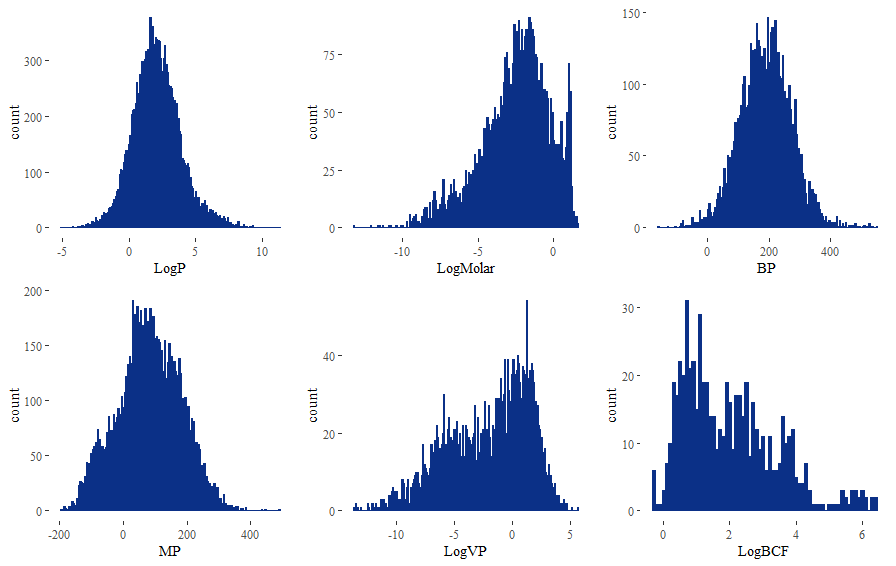
\includegraphics[scale=0.65]{properties.png}
\end{figure}

Summaries of the values for each physicochemical property are presented in Table 1.

\begin{table}[H]
\begin{center}
\begin{tabular}{lrrrrrrr}
\toprule
% \hline
&&\\
{\bf property} & {\bf N} & {\bf Min.} & {\bf 1st Qu.} &  {\bf Median}  & {\bf Mean}  & {\bf 3rd Qu.} & {\bf Max.}\\
% &&\\
%\hline
\midrule
&&\\
Log P  &  14026 & -5.08 & 0.89 & 2.00 & 2.08 & 3.16 & 11.29\\
Log S  &  4202 & -13.172 & -3.877 & -2.284 & -2.573 & -0.988 & 1.581\\
BP  &   5415 &-161.5 & 133.0 & 189.3 & 188.9 & 245.0 & 548.0\\
MP  &   8625& -196.00 & 16.00 & 80.00 & 80.45 & 151.20 & 492.50\\
VP  &   2701 & -13.6778 & -4.7696 & -1.2573 & -2.0395 & 0.8633 & 5.6682\\
BCF  &  626 &  -0.350 & 0.850 & 1.780 & 2.002 & 2.857 & 6.430\\
&&\\
%\hline
\bottomrule
\end{tabular}
\end{center}
\caption{Summaries of physicochemical properties. \textbf{N}: number of observations; \textbf{Min.}: minimum value; \textbf{1st Qu.}: first quartile (25th percentile);
\textbf{Median}: median (50th percentile); \textbf{Mean}: mean (average); \textbf{3rd Qu.}: third quartile (75th percentile);
\textbf{Max.}: maximum value.}
\end{table}


\subsection{Selection of Training Sets \& Test Sets}

The chemicals were randomly partitioned into training sets (75\% of the
chemicals) to build the models and test sets (25\% of the chemicals) to validate
the predictive power of each model. The property value distributions for these training sets and test sets are presented in Figure 2. That these distributions are coincident supports the assertion that training sets and test sets represent equivalent sample populations from the respective full datasets. Numerical summaries for property values in the training sets and test sets are presented in Table 2. The complementarity of these data summaries further speaks to the equivalence of the training sets and the test sets.

\begin{table}[H]
\begin{center}
\begin{tabular}{llrrrrrrr}
\toprule
{\bf property} & {\bf set} & {\bf N} & {\bf Min.} & {\bf 1st Qu.} &  {\bf Median}  & {\bf Mean}  & {\bf 3rd Qu.} & {\bf Max.}\\
\midrule
\multirow{2}{15mm}{Log P}
& train &  10520 & -5.080 & 0.890 & 2.000 & 2.075 & 3.160 & 11.290\\
& test &  3506 & -3.950 & 0.910 & 2.000 & 2.096 & 3.170 & 9.300\\
\midrule
\multirow{2}{15mm}{Log S}
& train &  3149 & -12.060 & -3.825 & -2.284 & -2.580 & -1.007 & 1.581\\
& test &  1063 & -13.172 & -3.929 & -2.284 & -2.553 & -0.945 & 1.541\\
\midrule
\multirow{2}{15mm}{BP}
& train &  4062 & -103.7 & 134.0 & 189.0 & 189.3 & 245.0 & 548.0\\
& test &  1353 & -161.5 & 131.0 & 190.5 & 187.5 & 244.5 & 512.0\\
\midrule
\multirow{2}{15mm}{MP}
& train &  6463 & -196.00 & 15.95 & 79.00 & 79.61 & 150.00 & 437.30\\
& test &  2162 & -187.60 & 16.62 & 83.00 & 82.97 & 156.88 & 492.50\\
\midrule
\multirow{2}{15mm}{VP}
& train &  2024 & -13.678 & -4.770 & -1.222 & -2.005 & 0.919 & 5.668\\
& test &  677 & -11.796 & -4.737 & -1.396 & -2.142 & 0.732 & 4.717\\
\midrule
\multirow{2}{15mm}{BCF}
& train &  469 & -0.300 & 0.860 & 1.800 & 2.006 & 2.820 & 6.360\\
& test &  157 & -0.350 & 0.780 & 1.700 & 1.990 & 2.960 & 6.430\\
\hline
\end{tabular}
\end{center}
\caption{Summaries of physicochemical properties for training and test sets. \textbf{N}: number of observations; \textbf{Min.}: minimum value; \textbf{1st Qu.}: first quartile (25th percentile);
\textbf{Median}: median (50th percentile); \textbf{Mean}: mean (average); \textbf{3rd Qu.}: third quartile (75th percentile);
\textbf{Max.}: maximum value.}
\end{table}

\begin{figure}
  \caption{Property value distributions for training sets and test sets.}
  \centering
    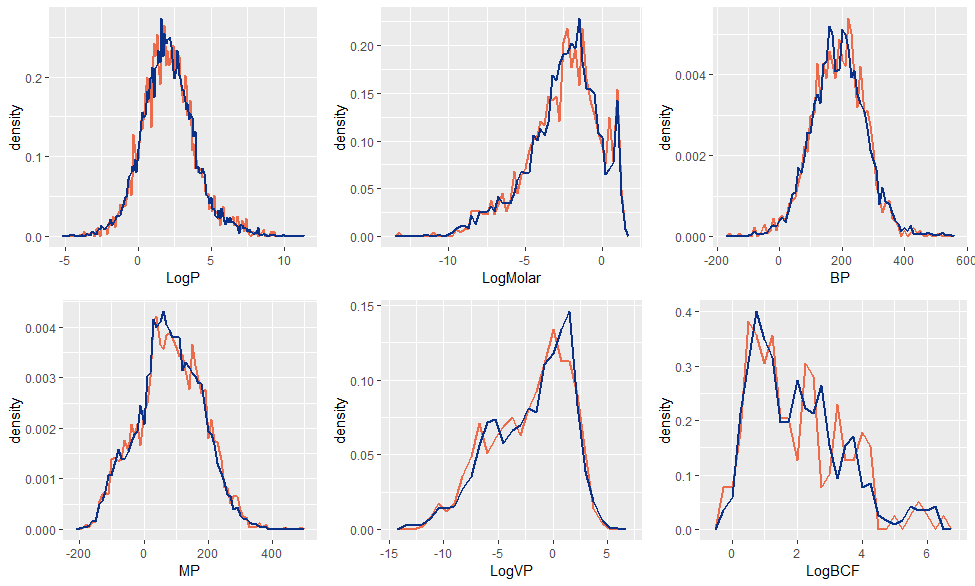
\includegraphics[width=1.0\textwidth]{TrainTestDensity.png}
\end{figure}

\subsection{Descriptor Calculation}

A key requirement for the predictive modeling of molecular properties and activities are molecular descriptors - numerical charaterizations of the molecular structure. The Chemistry Development Kit (CDK)\cite{CDK} was used to calculate molecular descriptors. The CDK is a collection of modular Java libraries for processing chemical information. It  implements a variety of molecular descriptors, categorized into topological, constitutional, geometric, electronic and hybrid\footnote{\burl{https://cdk.github.io/cdk/1.5/docs/api/org/openscience/cdk/qsar/descriptors/molecular/package-summary.html}}. The CDK was accessed using the R\cite{R} package rcdk\cite{rcdk}. This workflow, so constructed, guarantees reproducibility and scalability. In total, 115 1-dimensional and 2-dimensional descriptors are calculated for each molecule.

For each of the datasets, any descriptor having one unique value (\textit{i.e.}, zero variance descriptors) is removed. These descriptors have no information, and are discarded without consequence.

Further, highly correlated descriptors are removed. Redundant descriptors often add more complexity to a model than information they provide to the model. Using highly correlated descriptors -- in techniques like linear regression -- can result in highly unstable models, numerical errors, and degraded predictive performance. In these studies we've chosen a cutoff = 0.85; a minimum nimber of descriptors is removed to ensure that the absolute value of all pairwise correlations is below 0.85.

Table 3 reports the number of zero variance and highly correlated descriptors removed from each dataset, prior to modeling.

\begin{table}[H]
\begin{center}
\begin{tabular}{lrrr}
\toprule
% \hline
&&\\
{\bf property} & {\bf  \# Zero Variance} & {\bf \# Highly Correlated} & {\bf \# Descriptors Remaining}\\
% &&\\
%\hline
\midrule
&&\\
Log P  &  9 & 32 & 74\\
Log S  &  9 & 34 & 72\\
BP  &  10 & 39 & 66\\
MP  & 4 & 34 & 77\\
VP  & 11 & 37 & 67\\
BCF  & 11 & 34 & 70\\
&&\\
%\hline
\bottomrule
\end{tabular}
\end{center}
\caption{Summary of the number of zero variance and highly correlated descriptors removed from each dataset, prior to modeling}
\end{table}

\subsection{Model Development}

Each dataset was modeled using five machine learning algorithms: multiple linear regression (MLR), partial least squares regression (PLS), support vector machines (SVM), k-nearest neighbors (k-NN), and gradient boosted machines (gbm). Each of these algorithms is briefly described in the Supplement to this report. Each model was subjected to 5-fold cross-validation.

\subsection{Model Validation.} The performance of each QSPR model  
was evaluated by calculating the adjusted \( R^2\) from a linear model of predicted value versus experimental value.

\subsection{Applicability Domain}

\textbf{Applicability Domain.} The applicability domain (AD) of a QSPR model is the molecule space a model can
reliably predict. QSPR models are built using molecules in a training set. The applicability of these models towards reliable predictions is confined to those molecules that are similar to the training molecules. The similarity is measured using the calculated molecular descriptors. A qualitative assessment of the AD was used throughout this study. This assessment is described below.

For each dataset, the reduced set of training set descriptors (non-zero variance, not highly correlated; the \textbf{\# Descriptors Remaining} column in Table 3) was subjected to a principal component transformation. This same transformation was applied to the reduced set of test set descriptors. The first two principal components of the training set and the test set are plotted. The region(s) occupied by the training set in this 2-dimensional plot represent the applicability domain. To the degree that the test set points fall within this region, the test set falls within the applicability domain. Test set points falling outside this region are outside the applicability domain, and may not be well modeled.

The applicability domain plots for the six data sets are shown in Figure 3. There is considerable complementarity (overlap) in five of the six datasets. It is only for the bioconcentration factor dataset that one observes test dataset observations well outside the applicability domain. One possible consequence will be commented on later in this report.

\begin{figure}[H]
  \caption{Applicability domain plots. The applicability domain is represented by the training dataset (cyan points). The test dataset (light red points) is projected \textit{onto} the applicability domain.}
  \centering
    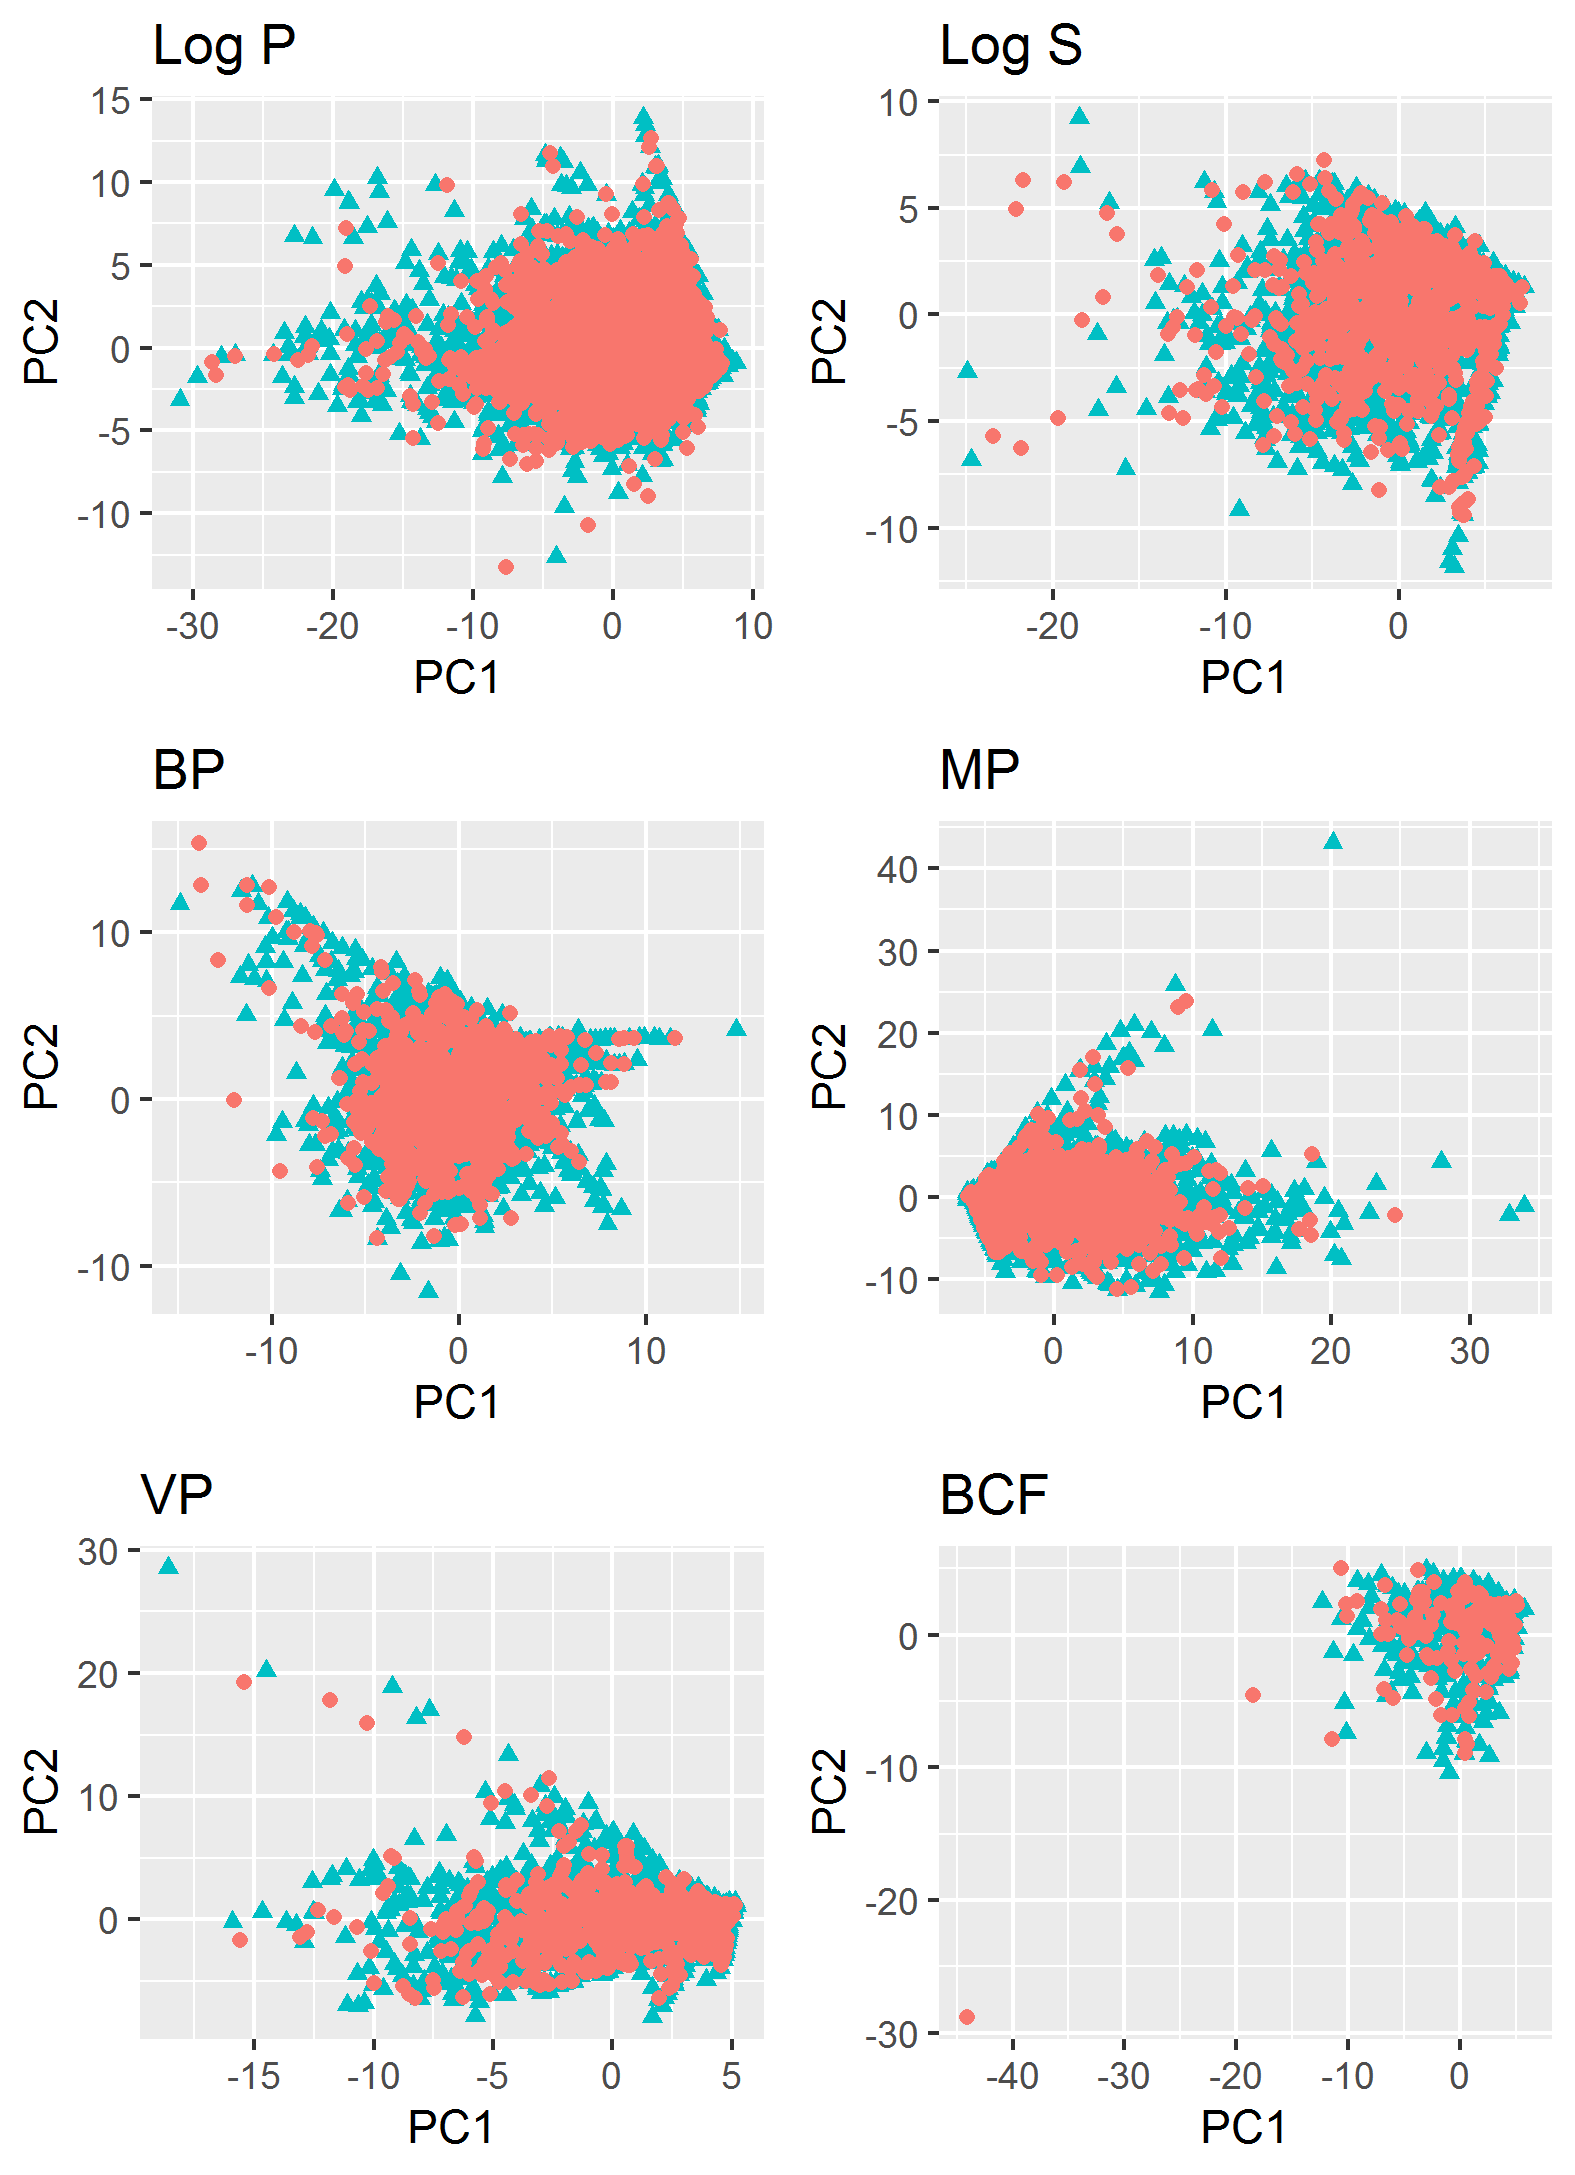
\includegraphics[scale=1.0]{PC_plots.png}
\end{figure}


\section{Results \& Discussion}

The results are summarized in Table 4. Gradient boosted machines (gbm) outperformed the other four approaches in predicting log P, log S,
 BP, MP, and BCF, as measured using the adjusted \( R^2\). In the case of VP, the adjusted \( R^2\) for SVM (0.9385) is only slightly better than the adjusted \( R^2\) for gbm (0.9327).

\begin{table}[H]
\begin{center}
\begin{tabular}{lrrrrr}
\toprule
% \hline
&&\\
{\bf property} & {\bf mlr} & {\bf pls} &  {\bf svm}  & {\bf kNN}  & {\bf gbm}\\
% &&\\
%\hline
\midrule
&&\\
Log P  &   0.8125 & 0.8098 & 0.9052 & 0.8546 & 0.9234\\
Log S  &   0.8317 & 0.8315 & 0.8770 & 0.8113 & 0.8924\\
BP  &   0.8978 & 0.8875 & 0.9487 & 0.8829 & 0.9535\\
MP  &   0.6849 & 0.6656 & 0.7841 & 0.7253 & 0.8106\\
VP  &   0.8834 & 0.8823 & 0.9385 & 0.8662 & 0.9327\\
BCF  &   0.0668 & 0.0398 & 0.7690 & 0.6916 & 0.8085\\
&&\\
%\hline
\bottomrule
\end{tabular}
\end{center}
\caption{Adjusted \( R^2\) for each model built in this study. \textbf{mlr}: multiple linear regression; \textbf{pls}: partial least squares regression; \textbf{svm}: support vector machine; \textbf{kNN}: k-nearest neighbors; \textbf{gbm}: gradient boosted machines. These machine learning algorithms are briefly described in the Supplement.}
\end{table}

The bioconcentration factor dataset is the \textit{least} accurately predicted across \textit{all} machine learning models. This is particularly true for multiple linear regression (\( R^2\) = 0.0668) and partial least squares (\( R^2\) = 0.0398). These two machine learning algorithms are sensitive to outliers. The applicability domain (AD) plot for this dataset (shown in Figure 3) shows observations in the test dataset falling outside the applicability domain, \textit{i.e.}, molecules that are \textit{dis}similar to the training set of molecules. If a test compound is considered outside a model’s applicability domain it cannot be associated with a reliable prediction, as is shown with the bioconcentration factor dataset.

\section{Conclusions}

Quantitative structure-property relationship (QSPR) models were developed for the
prediction of six physicochemical properties of environmental chemicals: octanol–water
partition coefficient (log P), water solubility (log S), boiling point (BP), melting point (MP),
vapor pressure (VP) and bioconcentration factor (BCF). The predictive accuracy of the models, as measured by the adjusted \( R^2\) between observed and predicted values for a hold-out test set, ranges from an adjusted \( R^2\) = 0.8085 (bioconcentration factor) to an adjusted \( R^2\) = 0.9535 (boiling point).

The data required to initiate a machine learning campaign is minimal. That data is
\begin{enumerate}
\item a representation of the molecule, or, information (\textit{e.g.}, compound name, CAS number, ...) that could be used to generate the representation, and
\item the endpoint (outcome) associated with the molecule.
\end{enumerate}
An example is presented in Table 5. Only one of \textbf{SMILES} or \textbf{NAME} is required. In this example, \textbf{Log BCF} is the endpoint.

\begin{table}[H]
\begin{center}
\begin{tabular}{llr}
%\toprule
% \hline
%&&\\
{\bf SMILES} & {\bf NAME} & {\bf Log BCF} \\
% &&\\
%\hline
\midrule
%&&\\
NC(N)=S  &   thiourea & 0.3 \\
Oc1c(Cl)cccc1Cl  &  2,6-dichlorophenol & 1.08 \\
CN(C)c1ccccc1  &  N,N-dimethylaniline & 0.9 \\
...  &  ... &  ... \\
%&&\\
%\hline
\bottomrule
\end{tabular}
\end{center}
\caption{Example input for ecotoxicological property prediction.}
\end{table}

There are opportunities available to Solvay colleagues:
\begin{itemize}
\item Colleagues interested in using one, a few, or all of the  models presented in this report to predict outcomes for their molecules should contact the author. Today, these models are provided as a service. Work is underway to build an interactive application that would afford  colleagues the opportunity to run these models from their desktop/laptop.
\item Colleagues interested in building a predictive model for data they have in-hand should also contact the author. As mentioned, requirements are minimal: (1) a representation of the molecule, and (2) the outcome associated with that molecule.
\end{itemize}

\newpage

\section{Supplemental Material}

\subsection{Machine Learning Algorithms}

\subsubsection{Multiple Linear Regression.} Multiple linear regression
(MLR) is widely used in the modeling of property data. We
used MLR to produce a linear model to describe the
relationship between a physicochemical property and the calculated
molecular descriptors:
\begin{equation}
property = \sum_{j = 1}^{m}c_{j}f_{j}
\end{equation}
In eq 7, \textit{property} is one of the six physicochemical properties
(logP, logS, logBCF, BP, MP or logVP); \(c_{j}\) is the contribution
coefficient, which is determined by regression analysis; and \(f_{j}\) is
the value of the jth descriptor. 

\subsubsection{Partial Least Squares Regression.} Partial least-squares
regression (PLSR) is a widely used multivariate analytical
technique in QSPR studies. The advantage of PLSR over
MLR lies in its ability to build a regression model based on
highly correlated descriptors, extract the relevant information,
and reduce data dimensions. We employed PLSR to generate
linear statistical models based on the calculated descriptors and the
physicochemical property being predicted. A set of orthogonal
latent variables or principal components (PCs) were first
generated through a linear combination of the original
descriptors, which served as new variables for
regression with the response variables (i.e., the physicochemical
properties) to build QSPR models. The optimal number of PCs
was determined by 10-fold cross-validation (CV).

\subsubsection{Support Vector Machines}
The basic concept of support vector regression is mapping the original data \textbf{X} nonlinearly into a higher dimensional feature space and solve a linear regression problem in this feature space.

\subsubsection{k-Nearest Neighbors}
The k-nearest neighbor algorithm (k-NN) is a method to classify objects based on closest examples in the feature space.
k-NN uses feature similarity to predict the value of any new data point. The new data point is assigned a vlue based on how closely that data point resembles points in the training set.

\subsubsection{Gradient Boosted Machines}
Gradient boosting is a machine learning technique for regression and classification problems, which produces a prediction model in the form of an ensemble of weak prediction models, typically decision trees. It builds the model in a stage-wise fashion like other boosting methods do, and it generalizes them by allowing optimization of an arbitrary differentiable loss function.

\newpage

\subsection{Physicochemical Property Modeling Summaries}

\subsubsection{Log P}

\begin{table}[H]
\begin{center}
\begin{tabular}{llrrrrrrr}
\toprule
{\bf property} & {\bf set} & {\bf N} & {\bf Min.} & {\bf 1st Qu.} &  {\bf Median}  & {\bf Mean}  & {\bf 3rd Qu.} & {\bf Max.}\\
\midrule
\multirow{2}{15mm}{Log P}
& train &  10520 & -5.080 & 0.890 & 2.000 & 2.075 & 3.160 & 11.290\\
& test &  3506 & -3.950 & 0.910 & 2.000 & 2.096 & 3.170 & 9.300\\
\midrule
\hline
\end{tabular}
\end{center}
\end{table}

\begin{figure}[H]
% \caption{Distributions of values for training sets and test sets.}
  \centering
    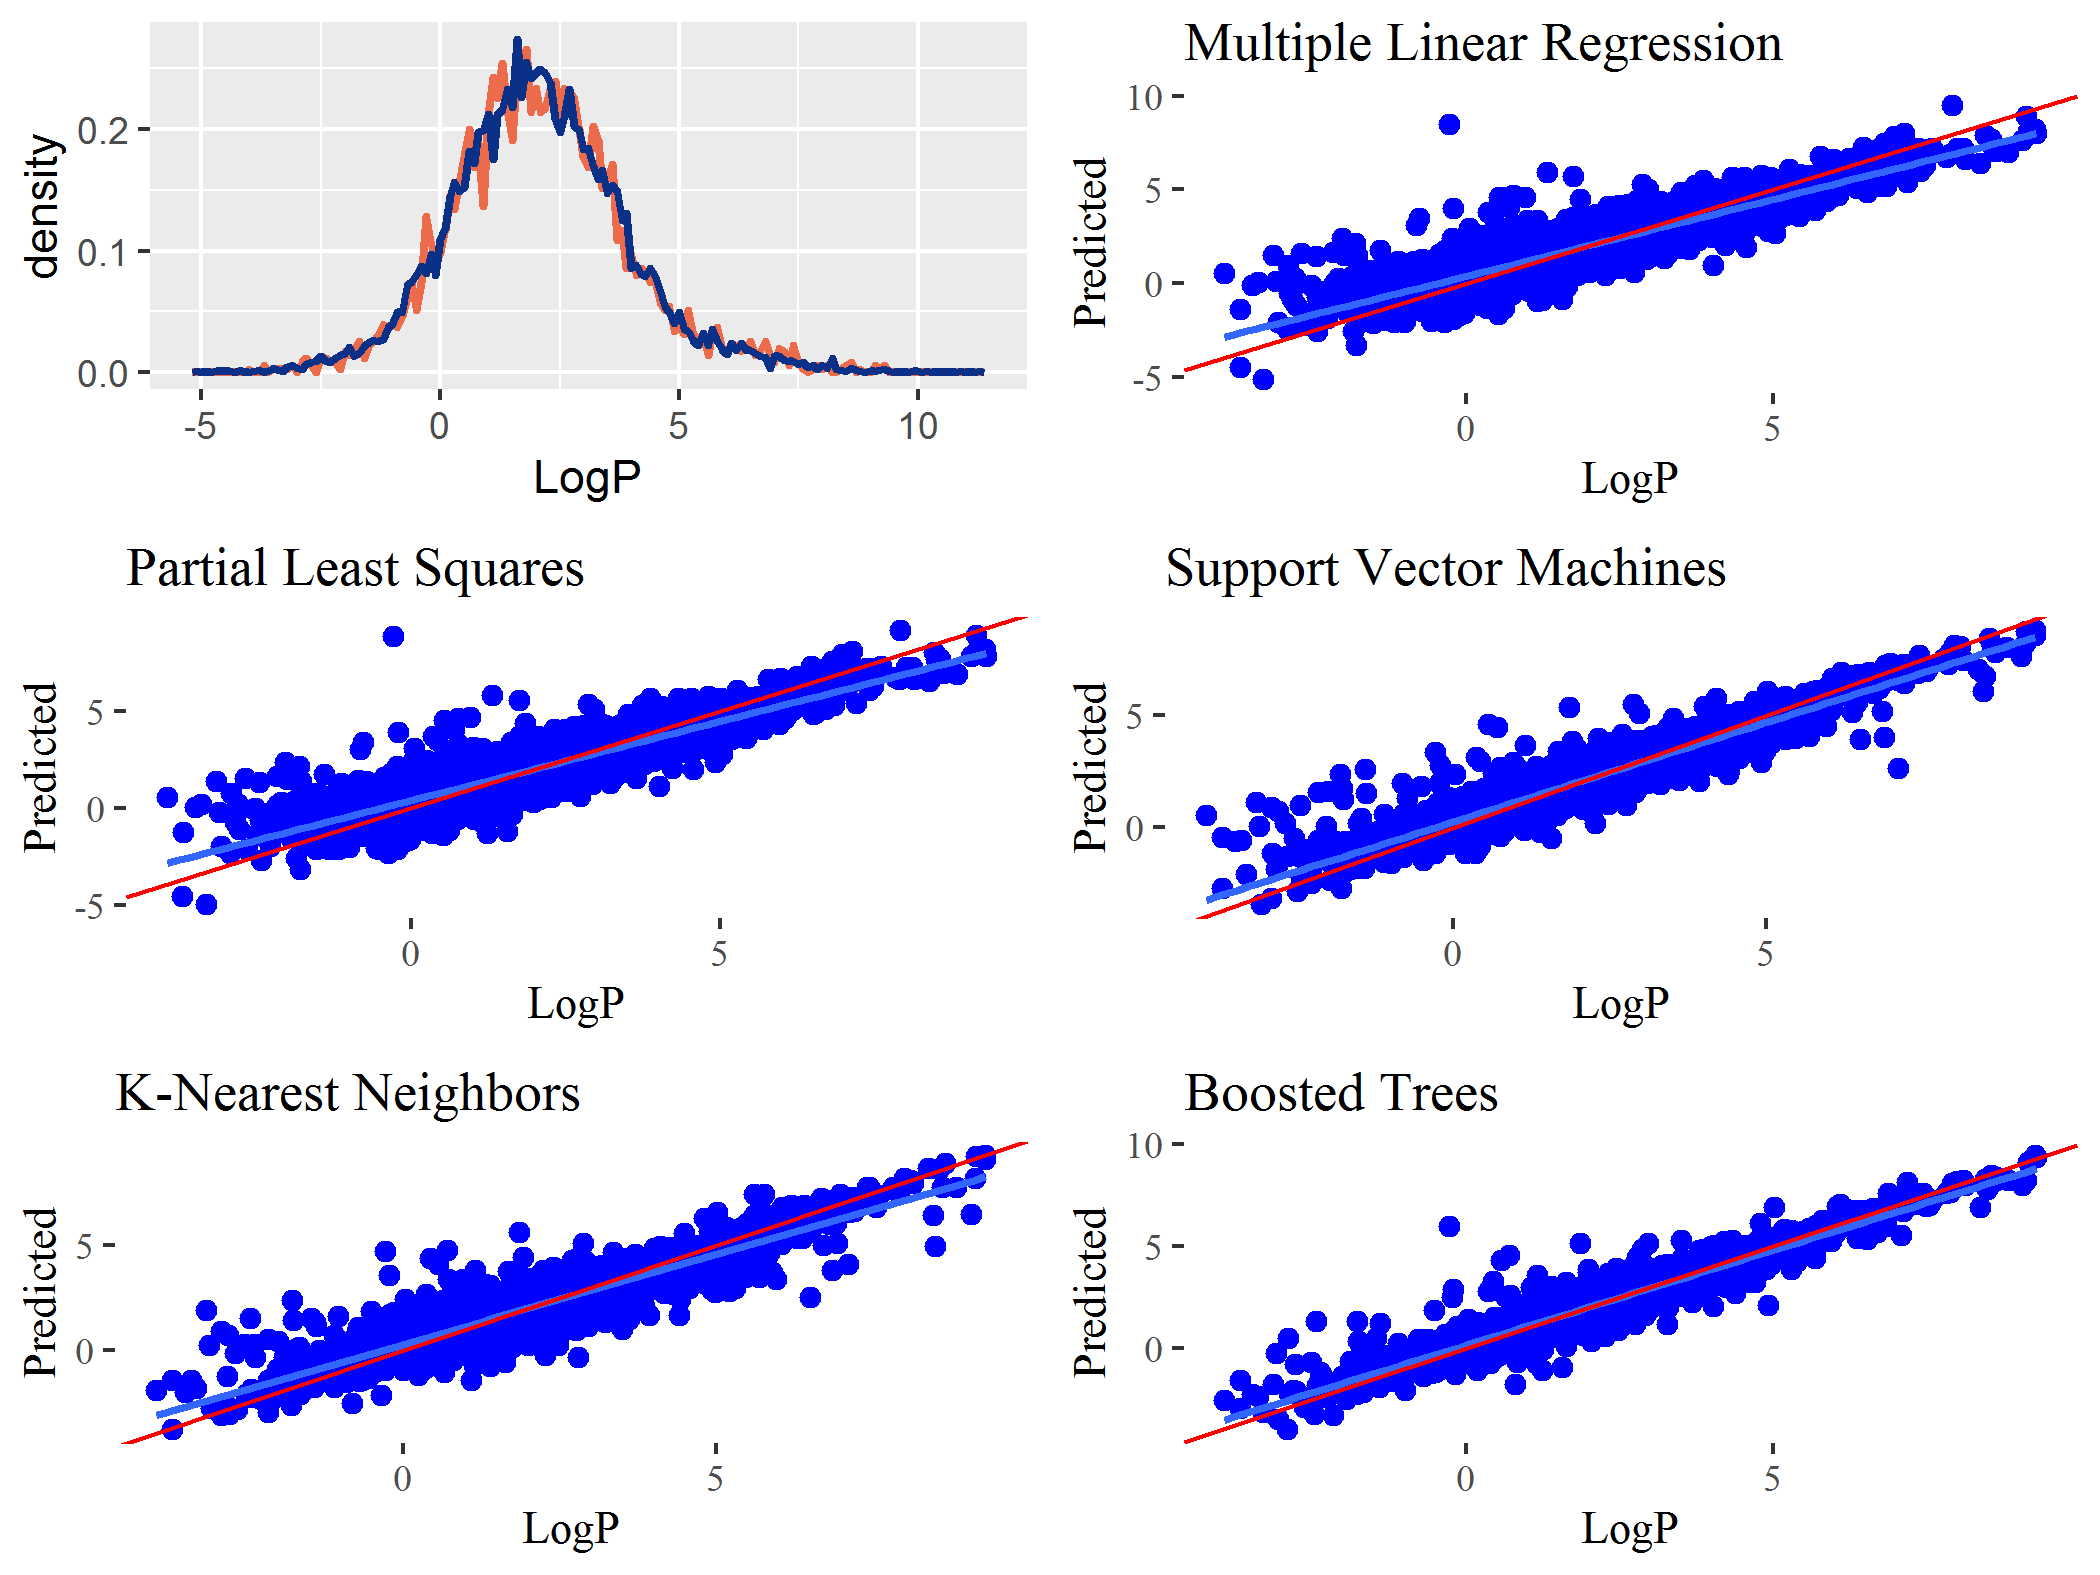
\includegraphics[width=1.0\textwidth]{LogP_plots.png}
\end{figure}

\begin{table}[H]
\begin{center}
\begin{tabular}{lrrrrr}
\toprule
% \hline
&&\\
{\bf property} & {\bf mlr} & {\bf pls} &  {\bf svm}  & {\bf kNN}  & {\bf gbm}\\
% &&\\
%\hline
\midrule
&&\\
Log P  &   0.8125 & 0.8098 & 0.9052 & 0.8546 & 0.9234\\
\midrule
\hline
%\bottomrule
\end{tabular}
\end{center}
%\caption{Adjusted \( R^2\).}
\end{table}

\subsubsection{Log S}

\begin{table}[H]
\begin{center}
\begin{tabular}{llrrrrrrr}
\toprule
{\bf property} & {\bf set} & {\bf N} & {\bf Min.} & {\bf 1st Qu.} &  {\bf Median}  & {\bf Mean}  & {\bf 3rd Qu.} & {\bf Max.}\\
\midrule
\multirow{2}{15mm}{Log S}
& train &  3149 & -12.060 & -3.825 & -2.284 & -2.580 & -1.007 & 1.581\\
& test &  1063 & -13.172 & -3.929 & -2.284 & -2.553 & -0.945 & 1.541\\
\midrule
\hline
\end{tabular}
\end{center}
\end{table}

\begin{figure}[H]
% \caption{Distributions of values for training sets and test sets.}
  \centering
    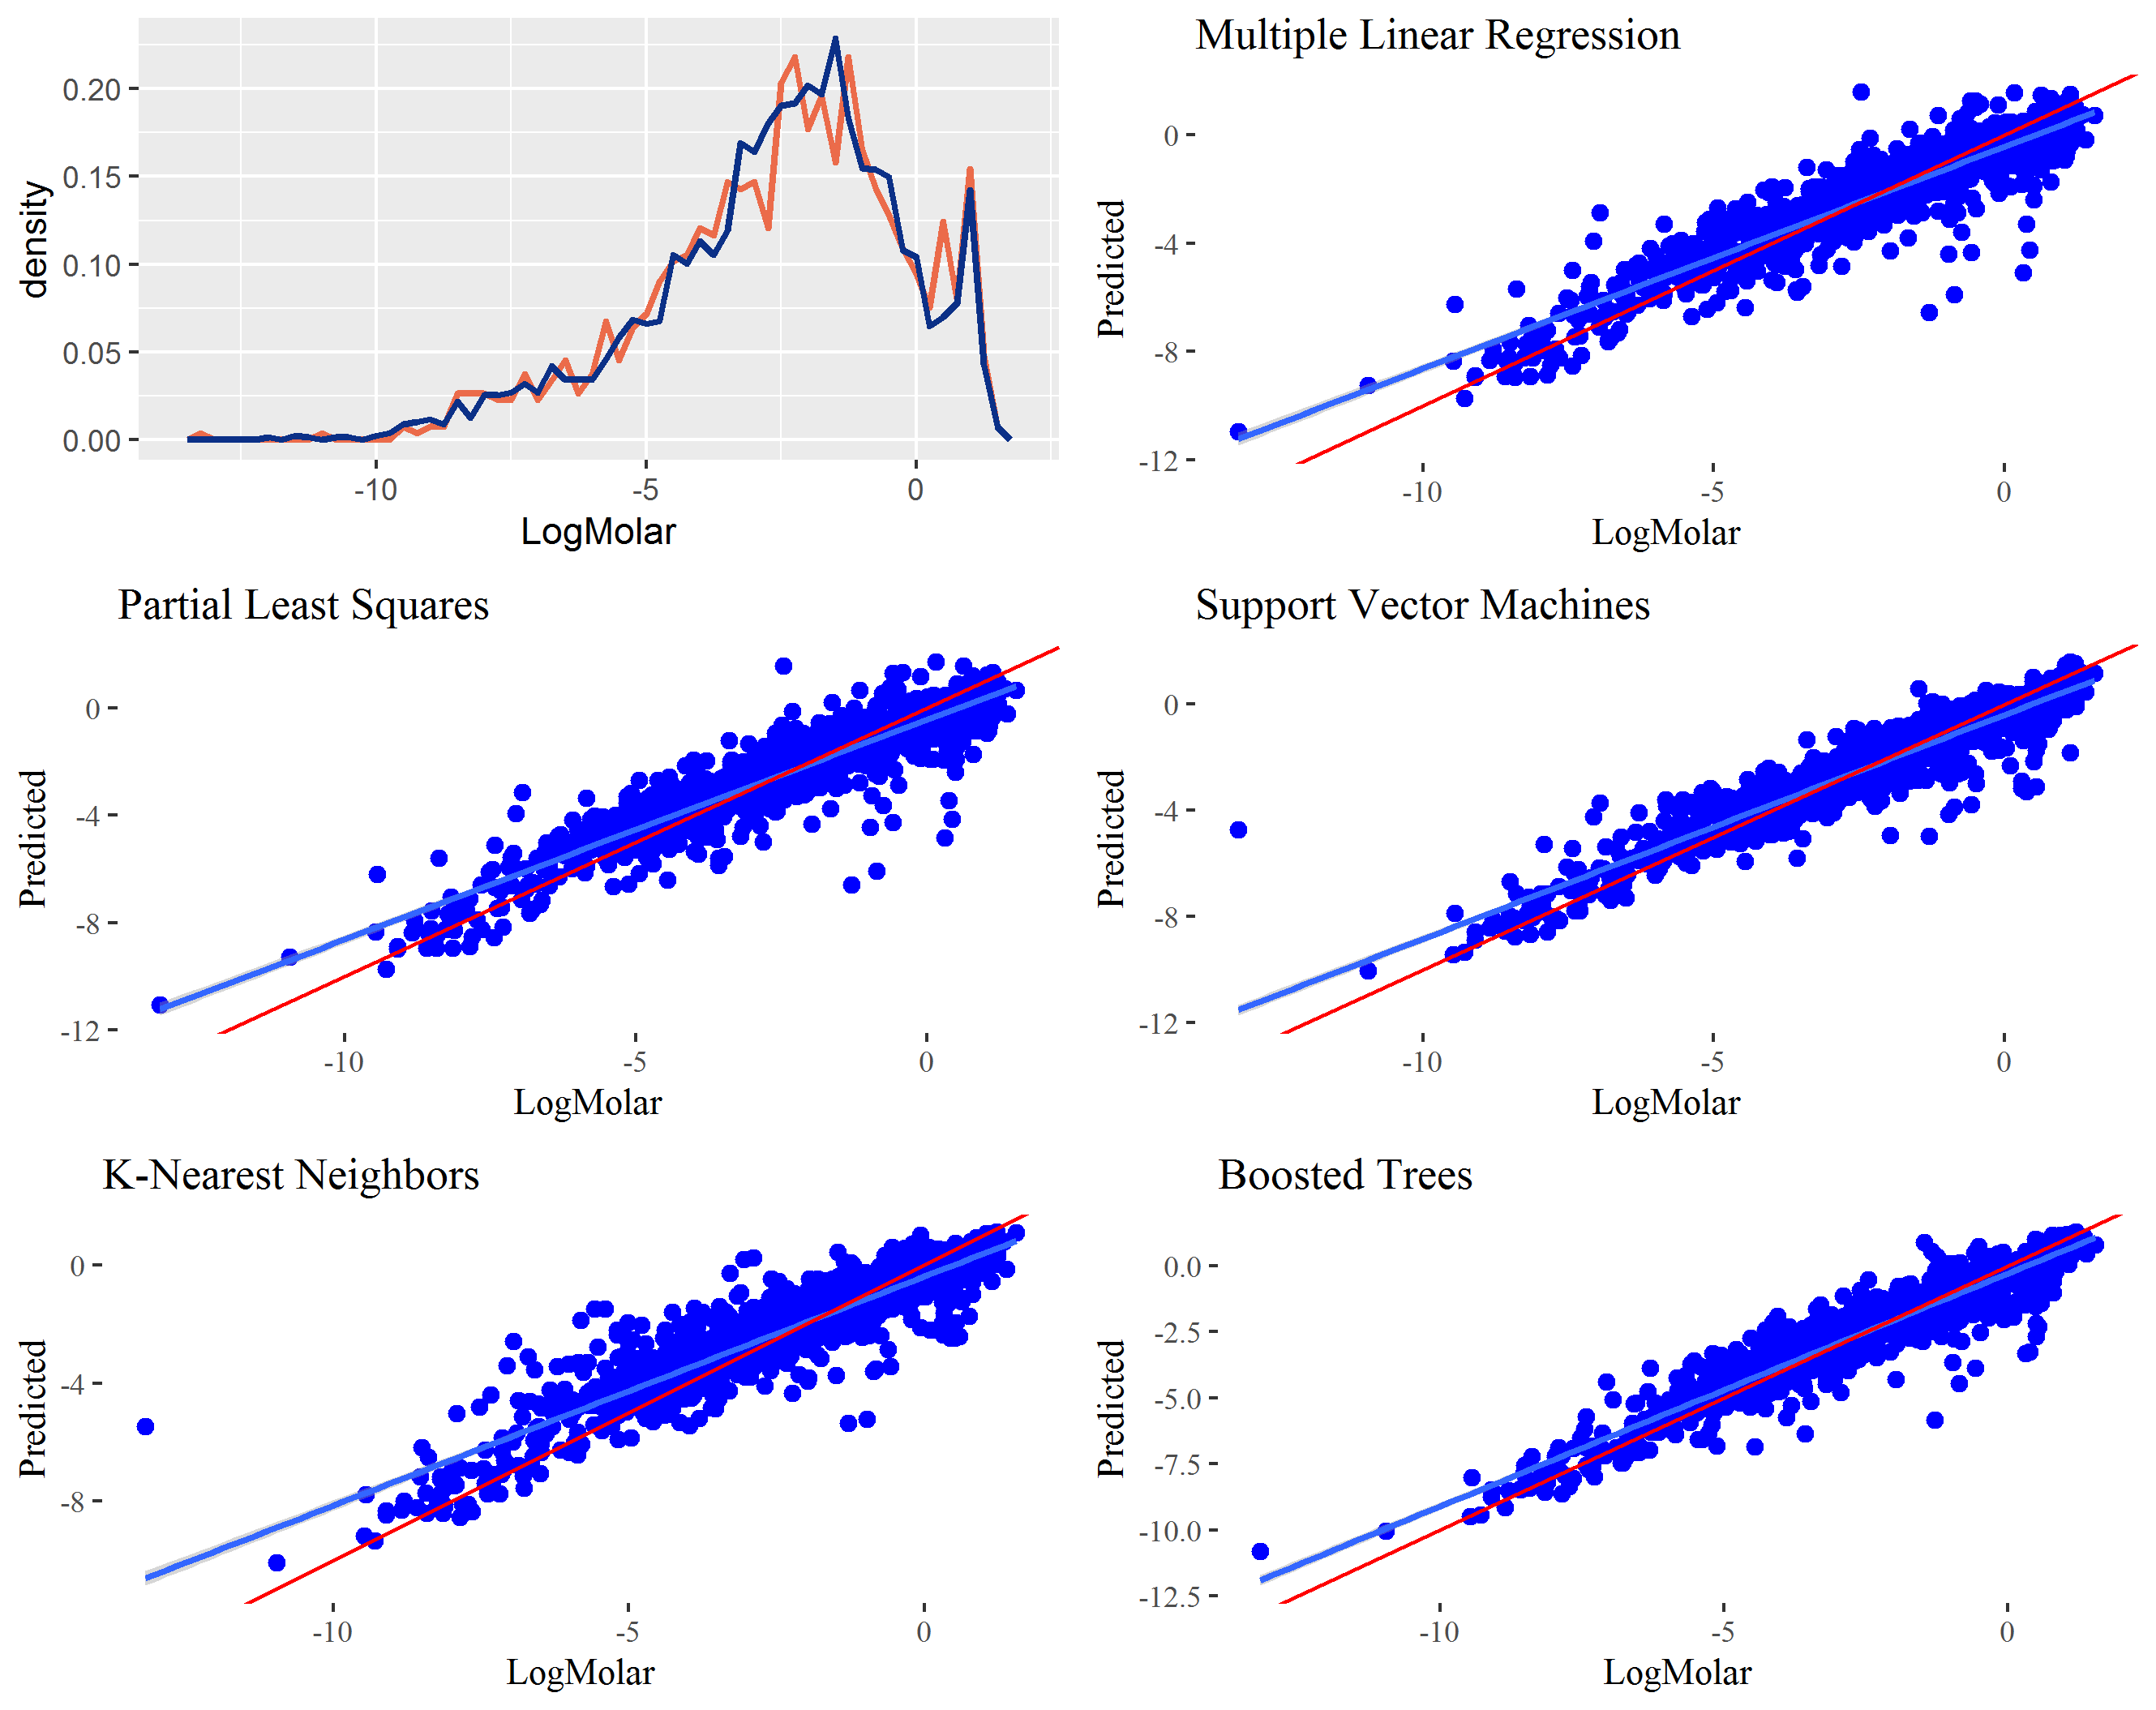
\includegraphics[width=1.0\textwidth]{LogMolar_plots.png}
\end{figure}

\begin{table}[H]
\begin{center}
\begin{tabular}{lrrrrr}
\toprule
% \hline
&&\\
{\bf property} & {\bf mlr} & {\bf pls} &  {\bf svm}  & {\bf kNN}  & {\bf gbm}\\
% &&\\
%\hline
\midrule
&&\\
Log S  &   0.8317 & 0.8315 & 0.8770 & 0.8113 & 0.8924\\
\midrule
\hline
%\bottomrule
\end{tabular}
\end{center}
%\caption{Adjusted \( R^2\).}
\end{table}

\subsubsection{Boiling Point}

\begin{table}[H]
\begin{center}
\begin{tabular}{llrrrrrrr}
\toprule
{\bf property} & {\bf set} & {\bf N} & {\bf Min.} & {\bf 1st Qu.} &  {\bf Median}  & {\bf Mean}  & {\bf 3rd Qu.} & {\bf Max.}\\
\midrule
\multirow{2}{15mm}{BP}
& train &  4062 & -103.7 & 134.0 & 189.0 & 189.3 & 245.0 & 548.0\\
& test &  1353 & -161.5 & 131.0 & 190.5 & 187.5 & 244.5 & 512.0\\
\midrule
\hline
\end{tabular}
\end{center}
\end{table}

\begin{figure}[H]
% \caption{Distributions of values for training sets and test sets.}
  \centering
    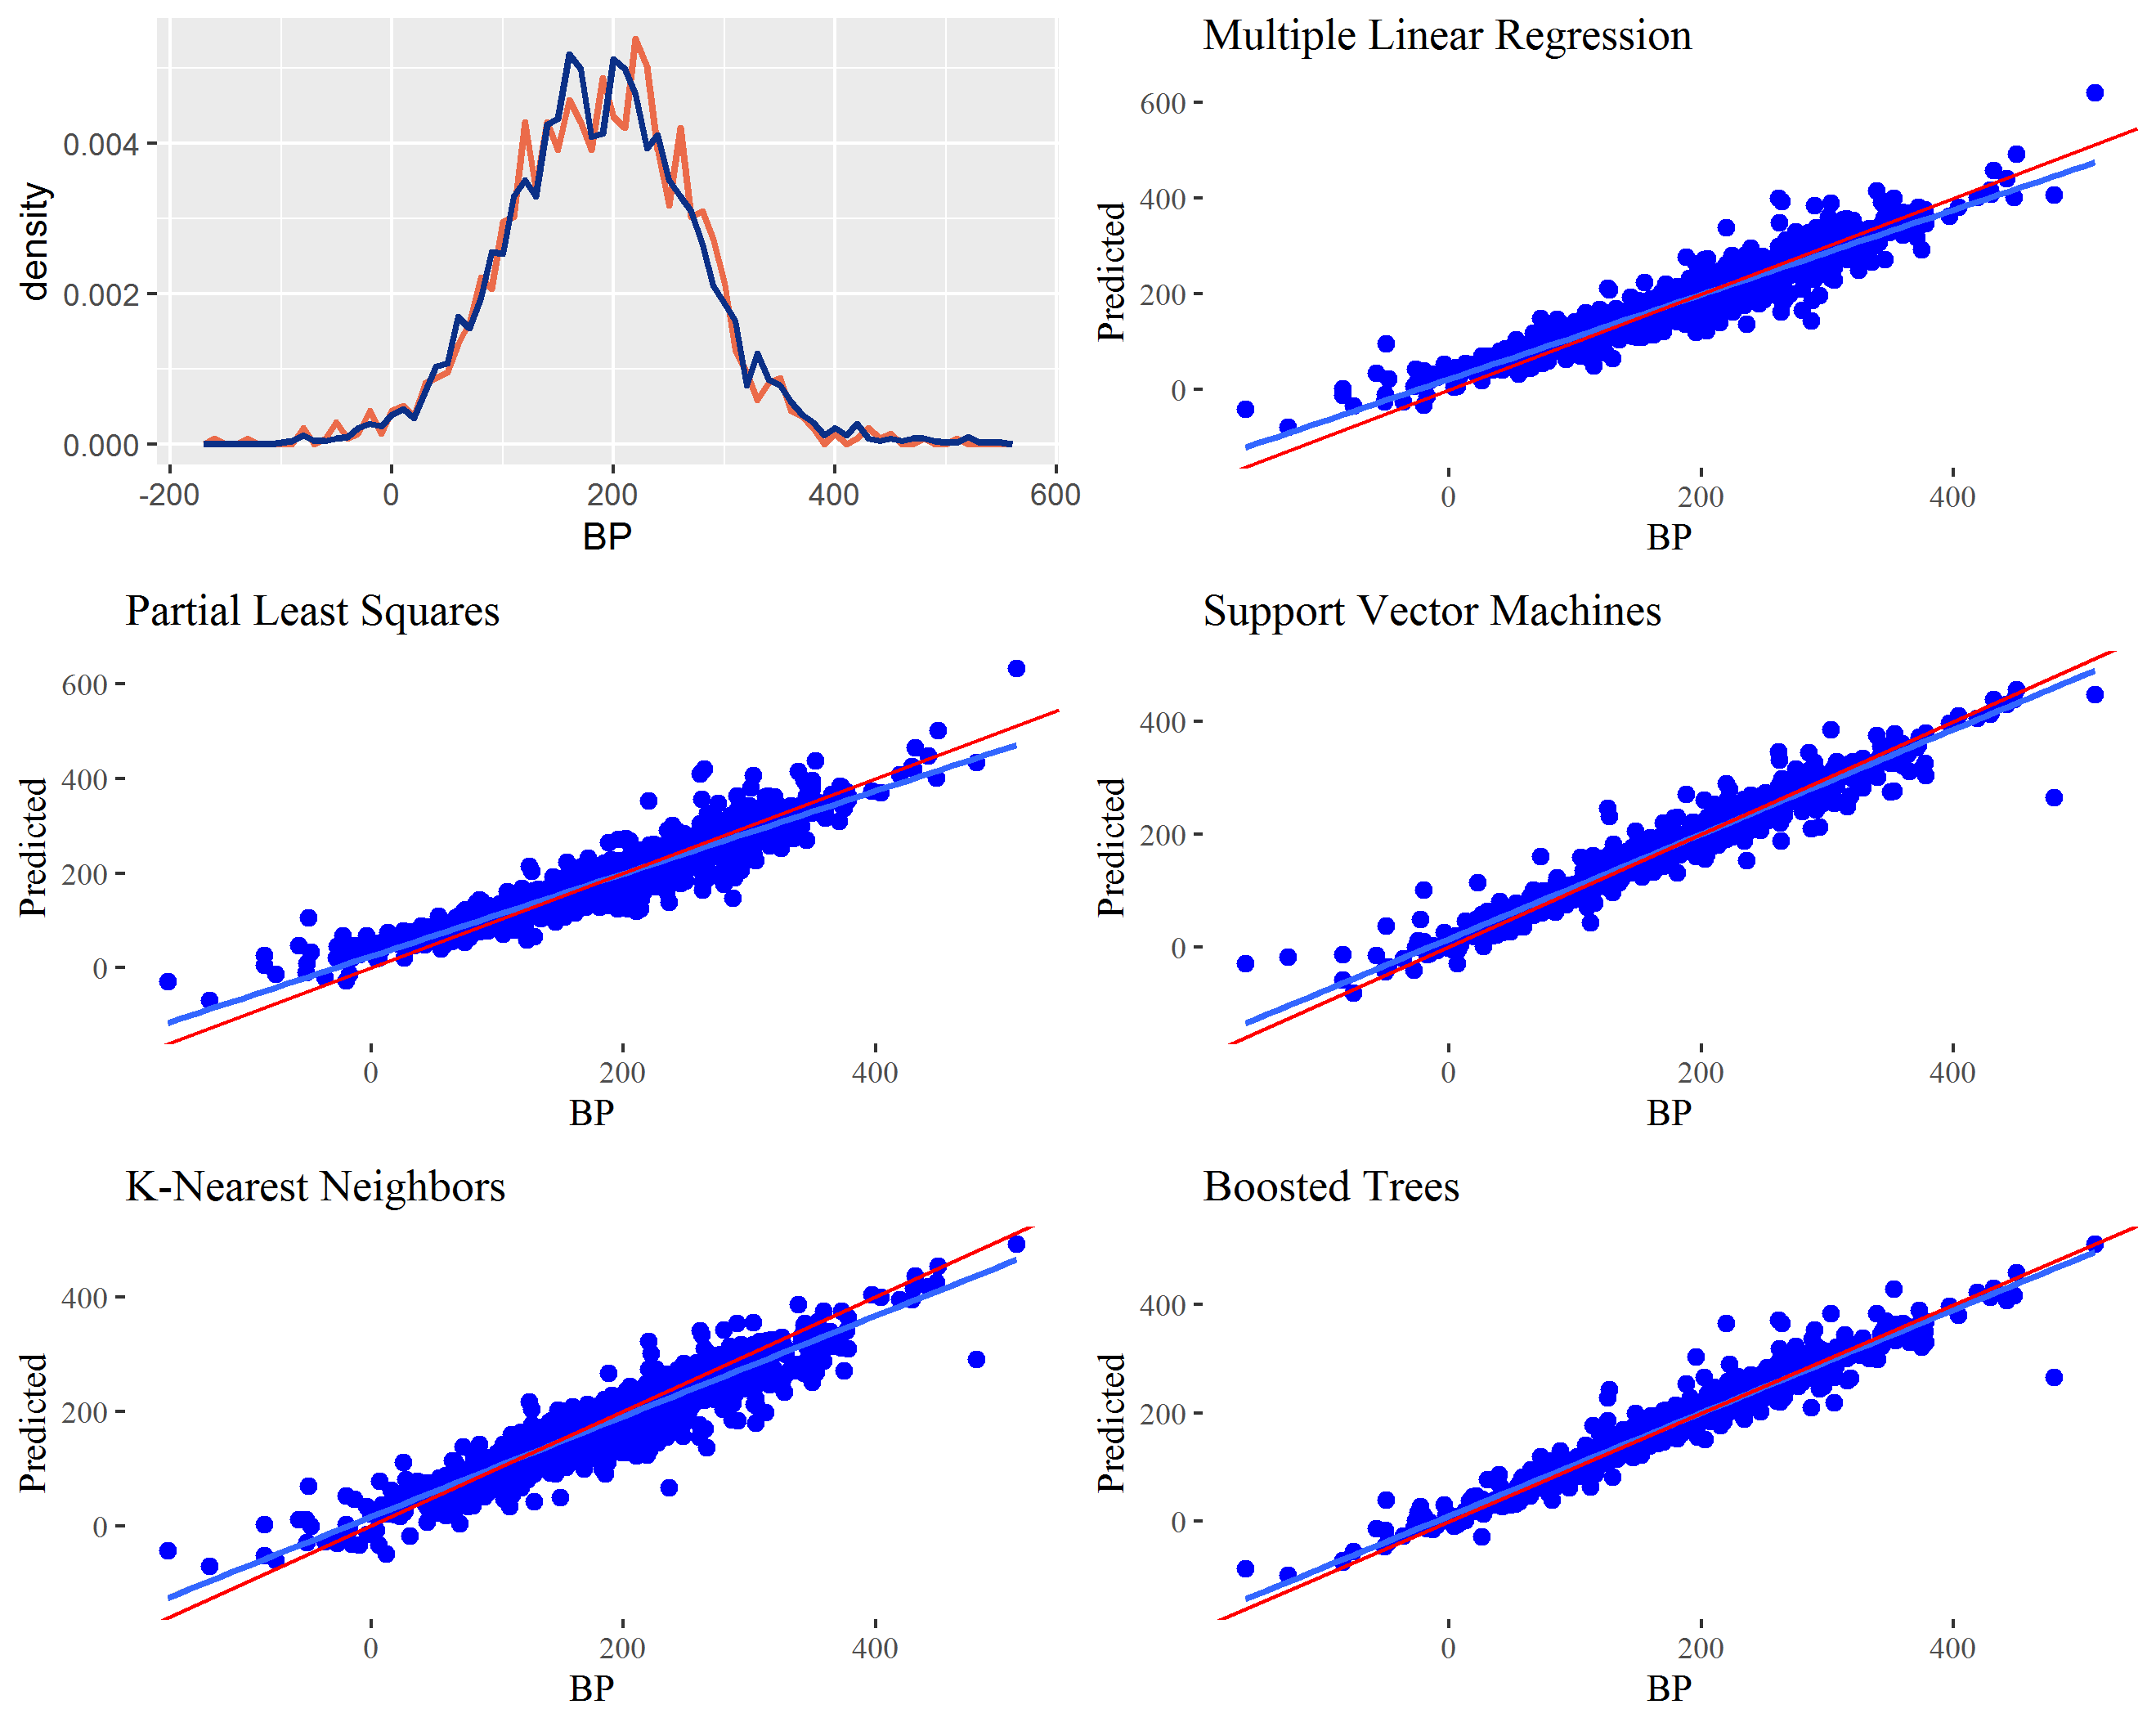
\includegraphics[width=1.0\textwidth]{BP_plots.png}
\end{figure}

\begin{table}[H]
\begin{center}
\begin{tabular}{lrrrrr}
\toprule
% \hline
&&\\
{\bf property} & {\bf mlr} & {\bf pls} &  {\bf svm}  & {\bf kNN}  & {\bf gbm}\\
% &&\\
%\hline
\midrule
&&\\
BP  &   0.8978 & 0.8875 & 0.9487 & 0.8829 & 0.9535\\
\midrule
\hline
%\bottomrule
\end{tabular}
\end{center}
%\caption{Adjusted \( R^2\).}
\end{table}

\subsubsection{Melting Point}

\begin{table}[H]
\begin{center}
\begin{tabular}{llrrrrrrr}
\toprule
{\bf property} & {\bf set} & {\bf N} & {\bf Min.} & {\bf 1st Qu.} &  {\bf Median}  & {\bf Mean}  & {\bf 3rd Qu.} & {\bf Max.}\\
\midrule
\multirow{2}{15mm}{MP}
& train &  6463 & -196.00 & 15.95 & 79.00 & 79.61 & 150.00 & 437.30\\
& test &  2162 & -187.60 & 16.62 & 83.00 & 82.97 & 156.88 & 492.50\\
\midrule
\hline
\end{tabular}
\end{center}
\end{table}

\begin{figure}[H]
% \caption{Distributions of values for training sets and test sets.}
  \centering
    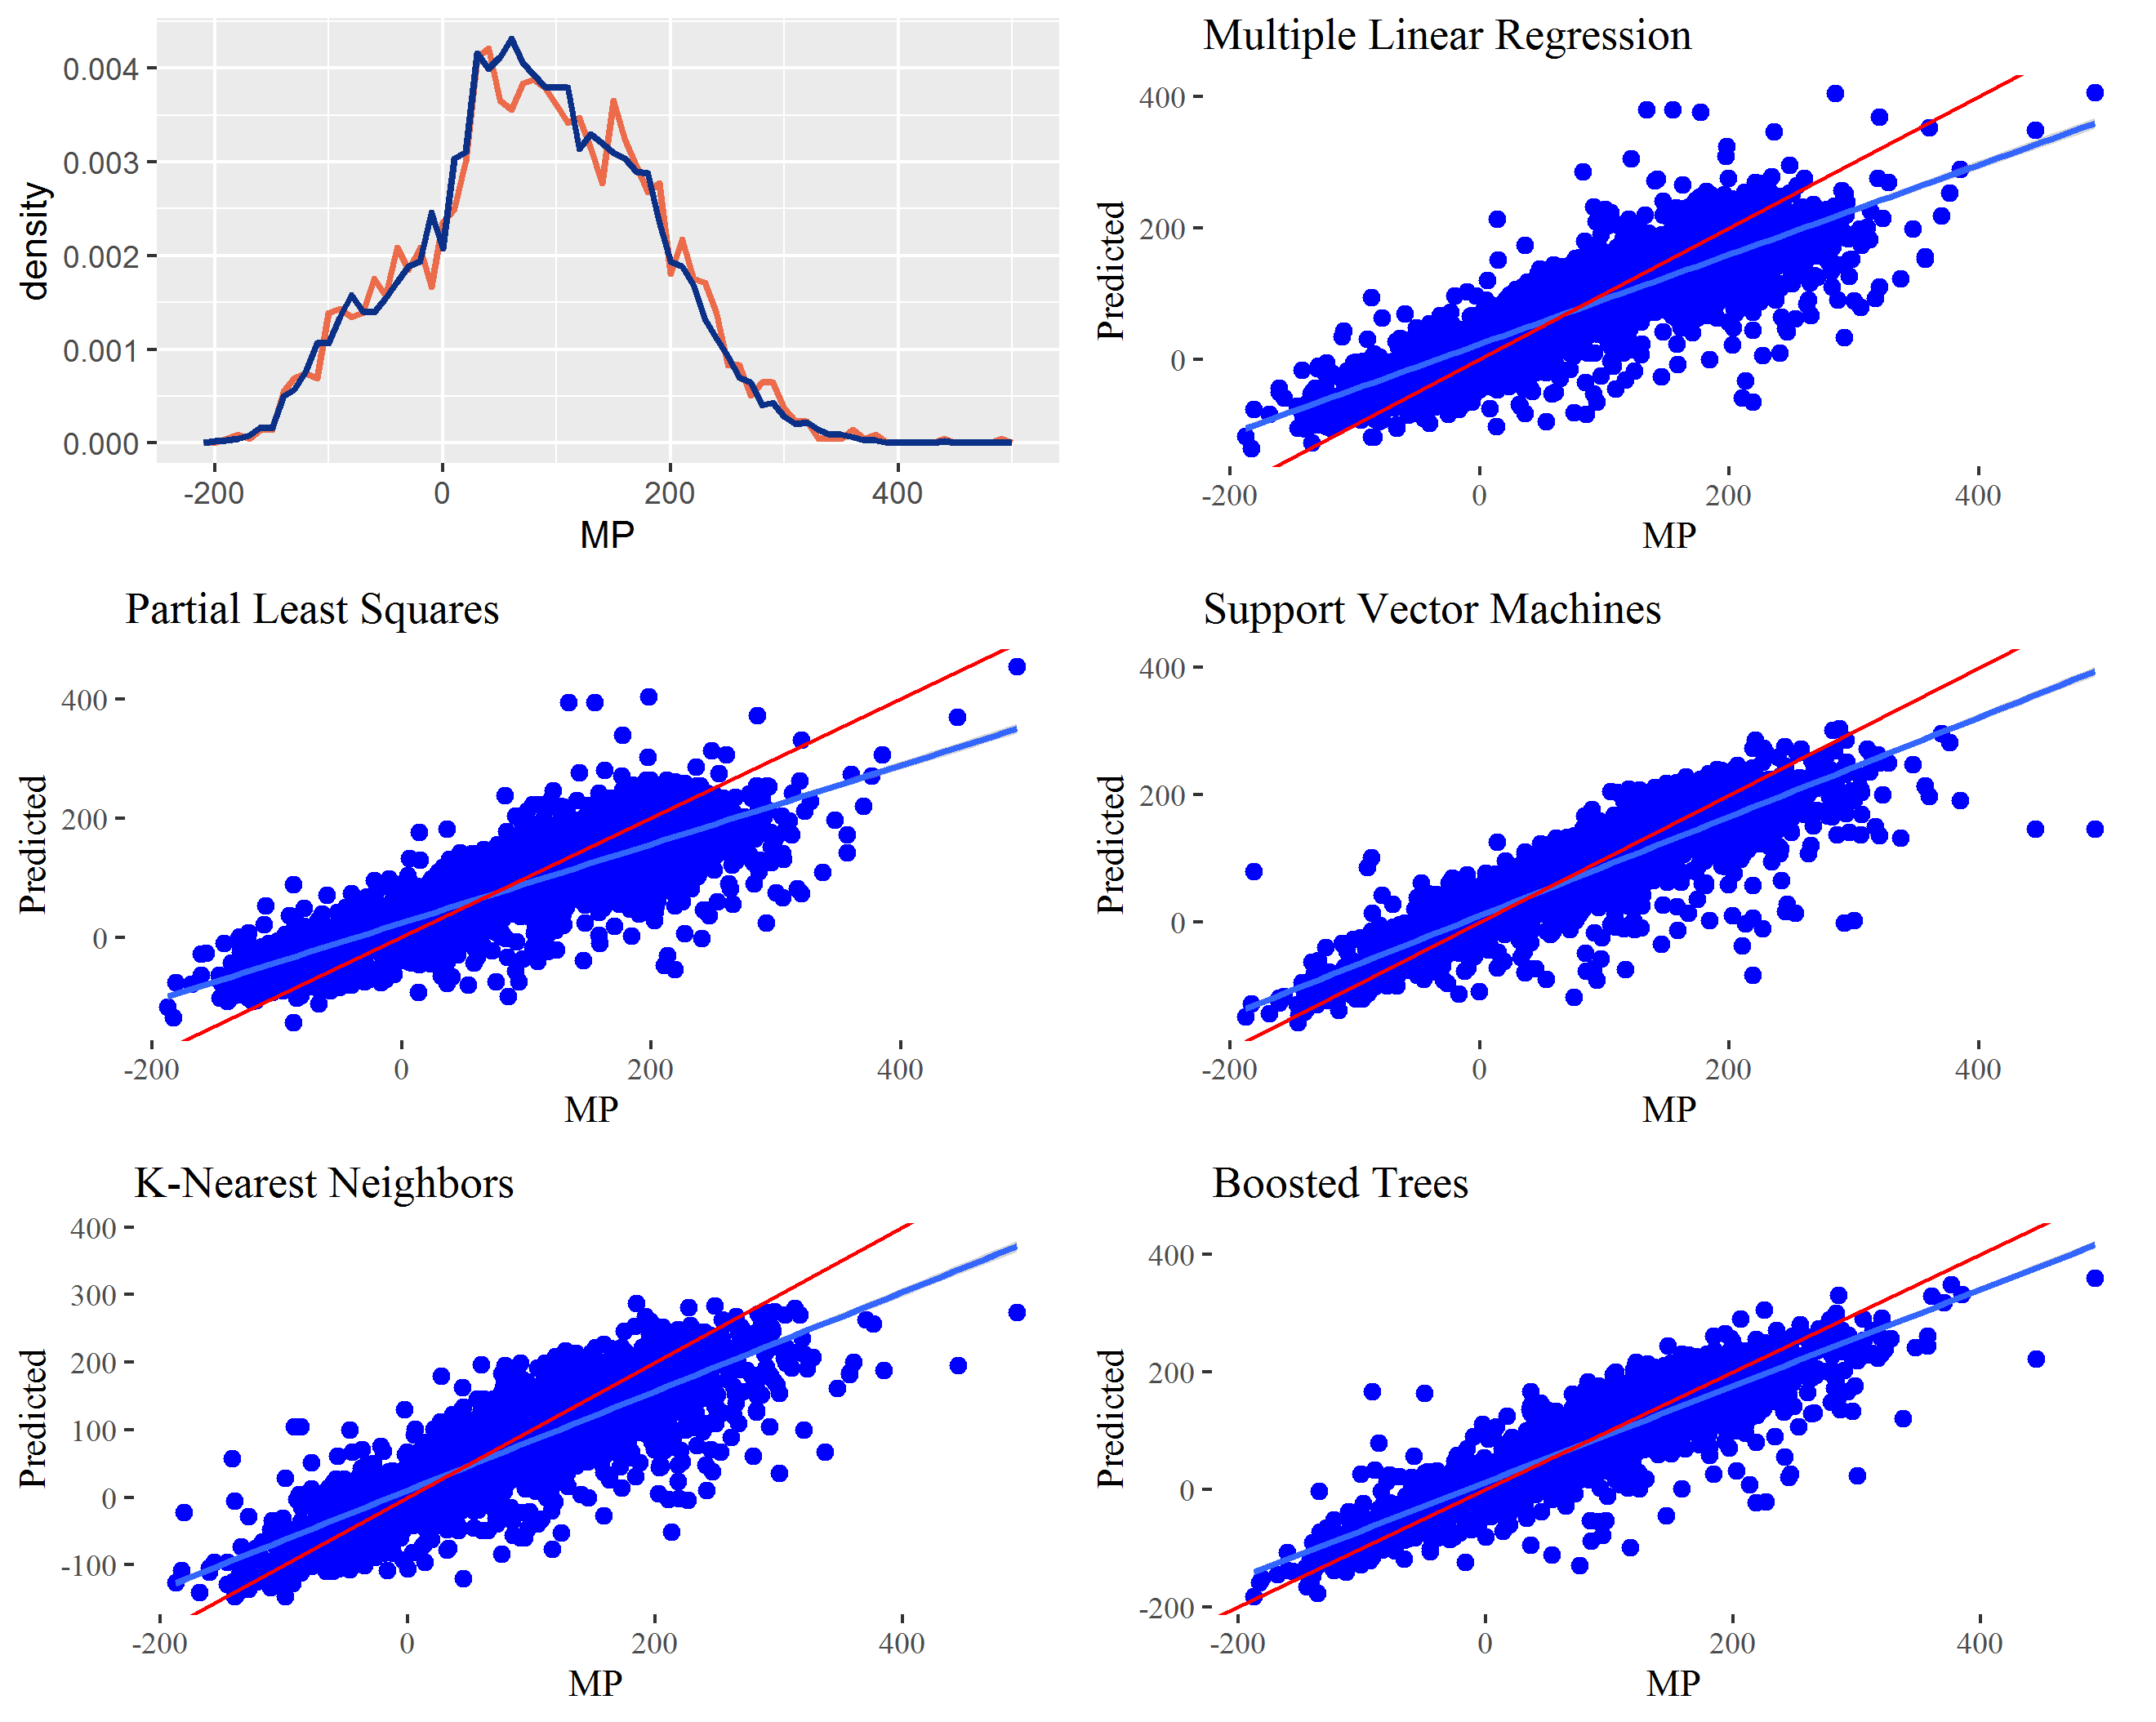
\includegraphics[width=1.0\textwidth]{MP_plots.png}
\end{figure}

\begin{table}[H]
\begin{center}
\begin{tabular}{lrrrrr}
\toprule
% \hline
&&\\
{\bf property} & {\bf mlr} & {\bf pls} &  {\bf svm}  & {\bf kNN}  & {\bf gbm}\\
% &&\\
%\hline
\midrule
&&\\
MP  &   0.6849 & 0.6656 & 0.7841 & 0.7253 & 0.8106\\
\midrule
\hline
%\bottomrule
\end{tabular}
\end{center}
%\caption{Adjusted \( R^2\).}
\end{table}

\subsubsection{Vapor Pressure}

\begin{table}[H]
\begin{center}
\begin{tabular}{llrrrrrrr}
\toprule
{\bf property} & {\bf set} & {\bf N} & {\bf Min.} & {\bf 1st Qu.} &  {\bf Median}  & {\bf Mean}  & {\bf 3rd Qu.} & {\bf Max.}\\
\midrule
\multirow{2}{15mm}{VP}
& train &  2024 & -13.678 & -4.770 & -1.222 & -2.005 & 0.919 & 5.668\\
& test &  677 & -11.796 & -4.737 & -1.396 & -2.142 & 0.732 & 4.717\\
\midrule
\hline
\end{tabular}
\end{center}
\end{table}

\begin{figure}[H]
% \caption{Distributions of values for training sets and test sets.}
  \centering
    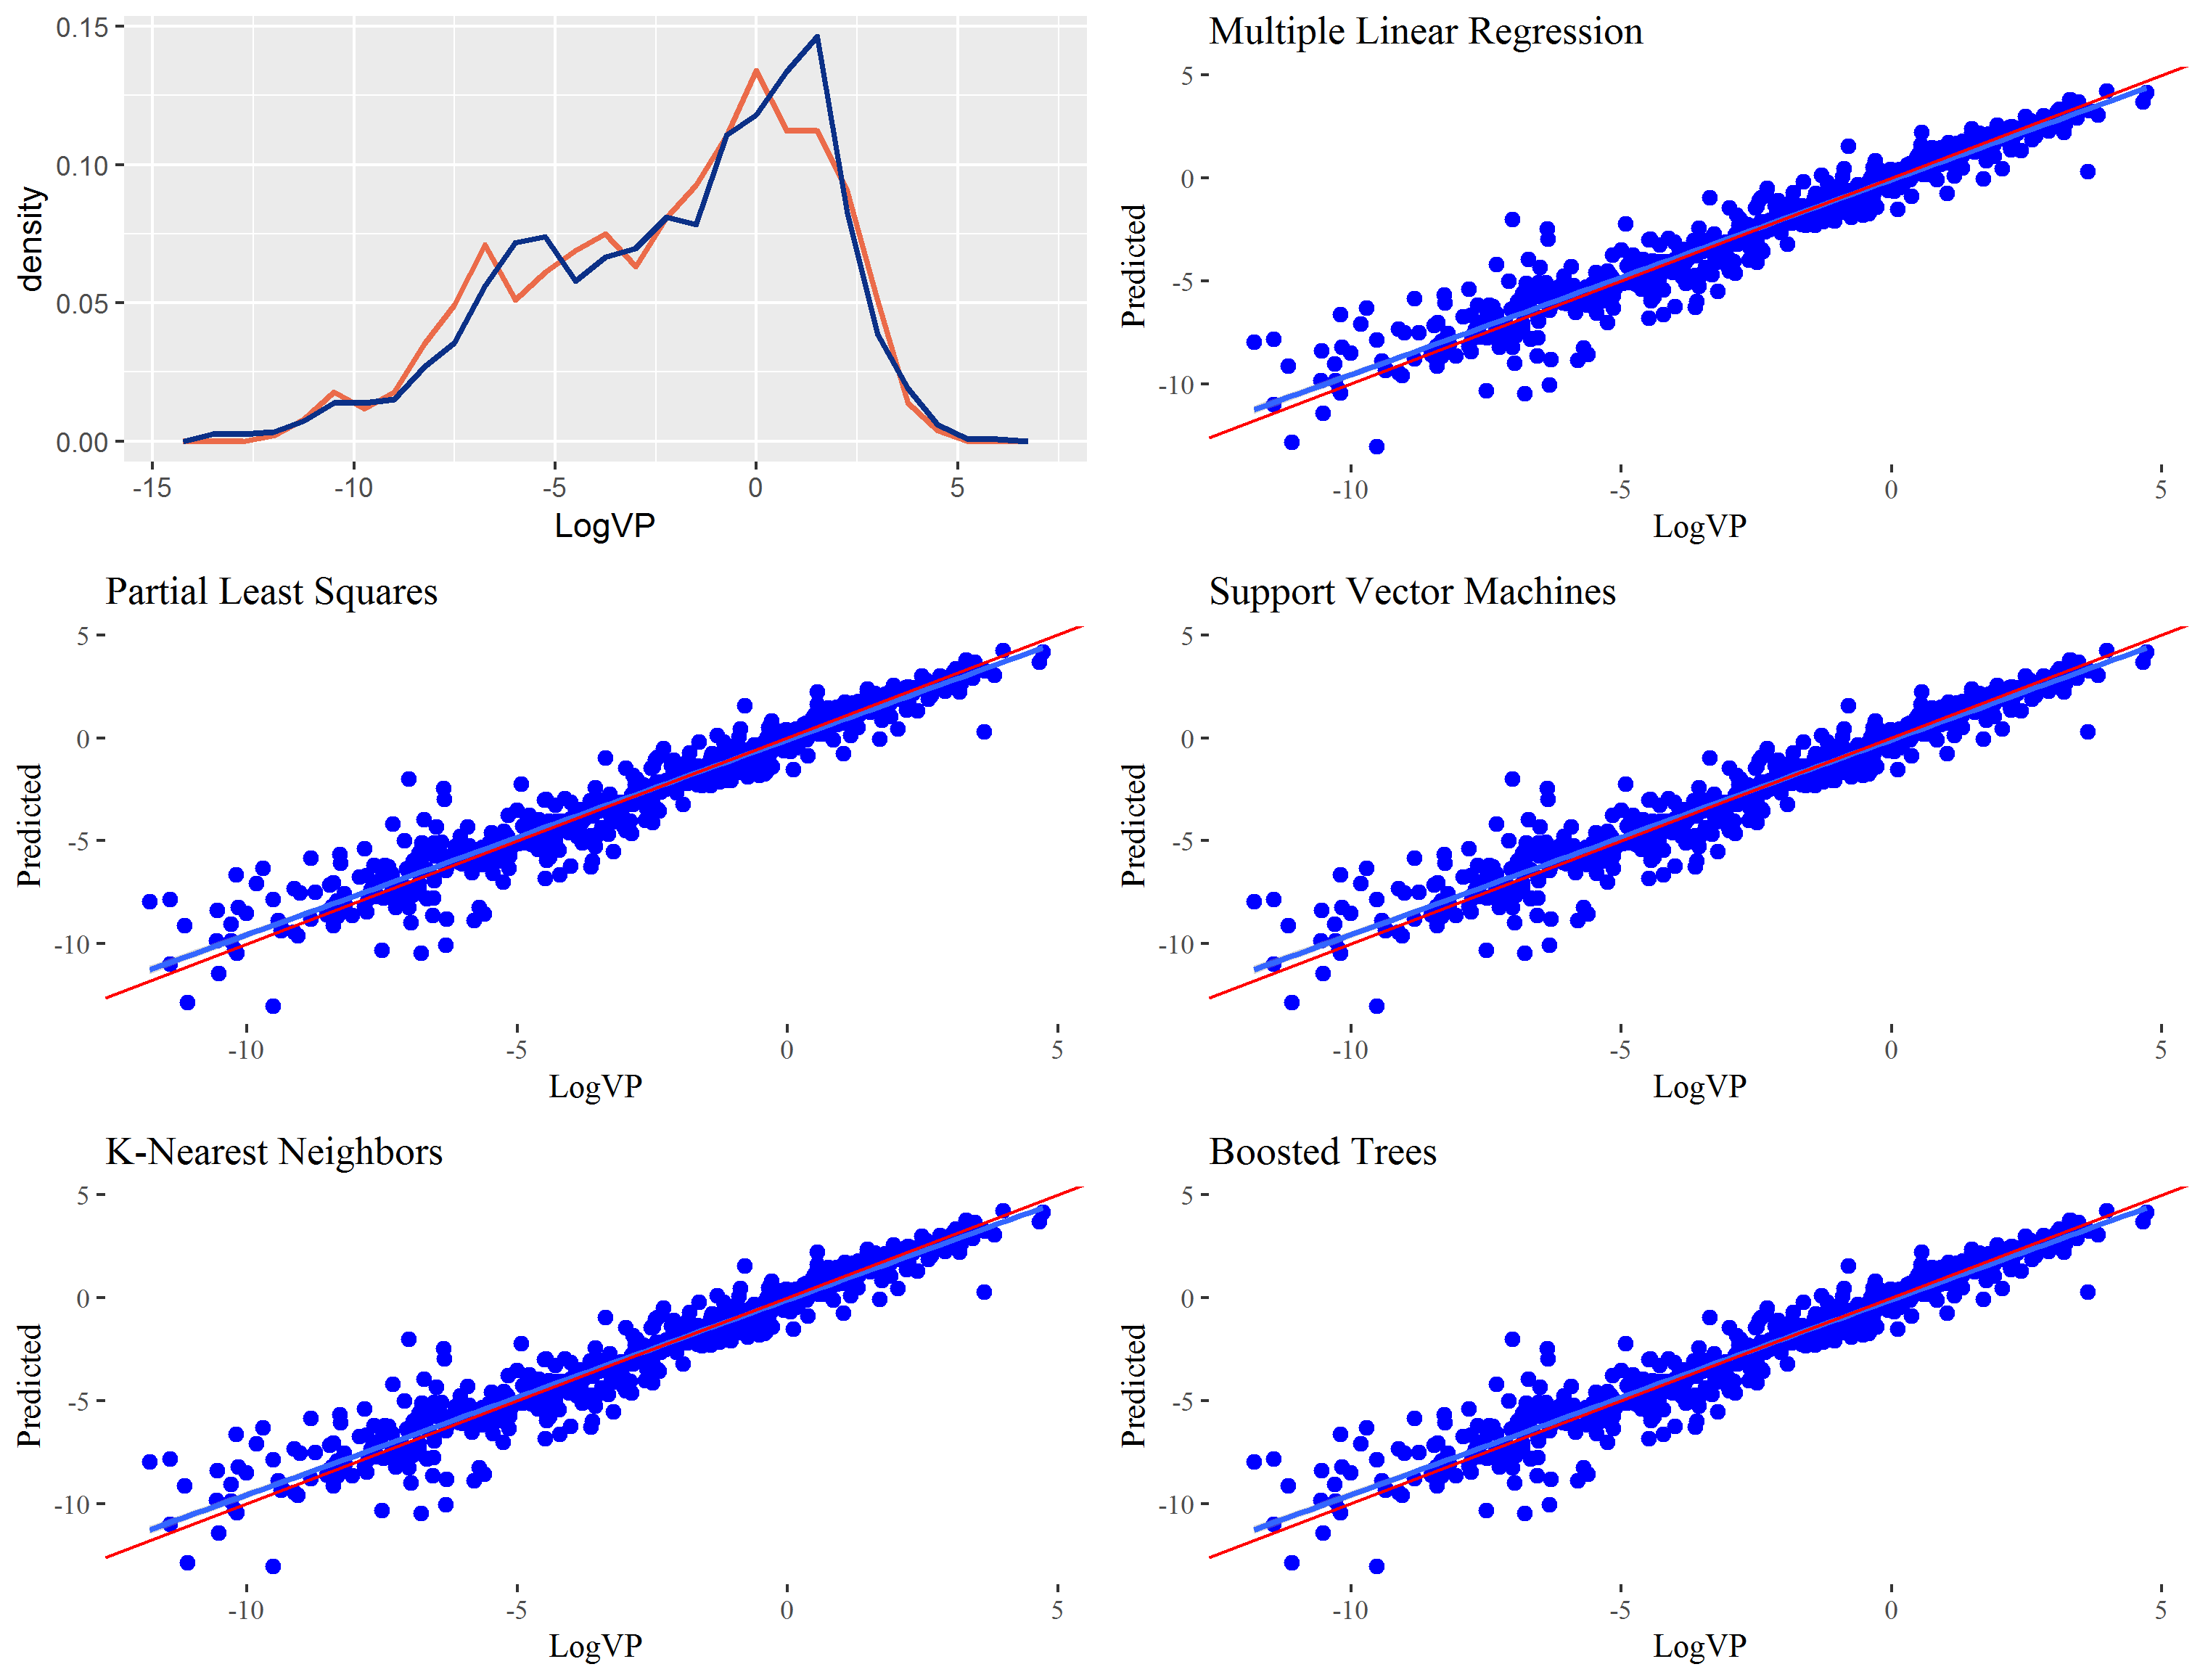
\includegraphics[width=1.0\textwidth]{VP_plots.png}
\end{figure}

\begin{table}[H]
\begin{center}
\begin{tabular}{lrrrrr}
\toprule
% \hline
&&\\
{\bf property} & {\bf mlr} & {\bf pls} &  {\bf svm}  & {\bf kNN}  & {\bf gbm}\\
% &&\\
%\hline
\midrule
&&\\
VP  &   0.8834 & 0.8823 & 0.9385 & 0.8662 & 0.9327\\
&&\\
\midrule
\hline
%\bottomrule
\end{tabular}
\end{center}
%\caption{Adjusted \( R^2\).}
\end{table}

\subsubsection{Bioconcentration Factor}

\begin{table}[H]
\begin{center}
\begin{tabular}{llrrrrrrr}
\toprule
{\bf property} & {\bf set} & {\bf N} & {\bf Min.} & {\bf 1st Qu.} &  {\bf Median}  & {\bf Mean}  & {\bf 3rd Qu.} & {\bf Max.}\\
\midrule
\multirow{2}{15mm}{BCF}
& train &  469 & -0.300 & 0.860 & 1.800 & 2.006 & 2.820 & 6.360\\
& test &  157 & -0.350 & 0.780 & 1.700 & 1.990 & 2.960 & 6.430\\
\midrule
\hline
\end{tabular}
\end{center}
\end{table}

\begin{figure}[H]
% \caption{Distributions of values for training sets and test sets.}
  \centering
    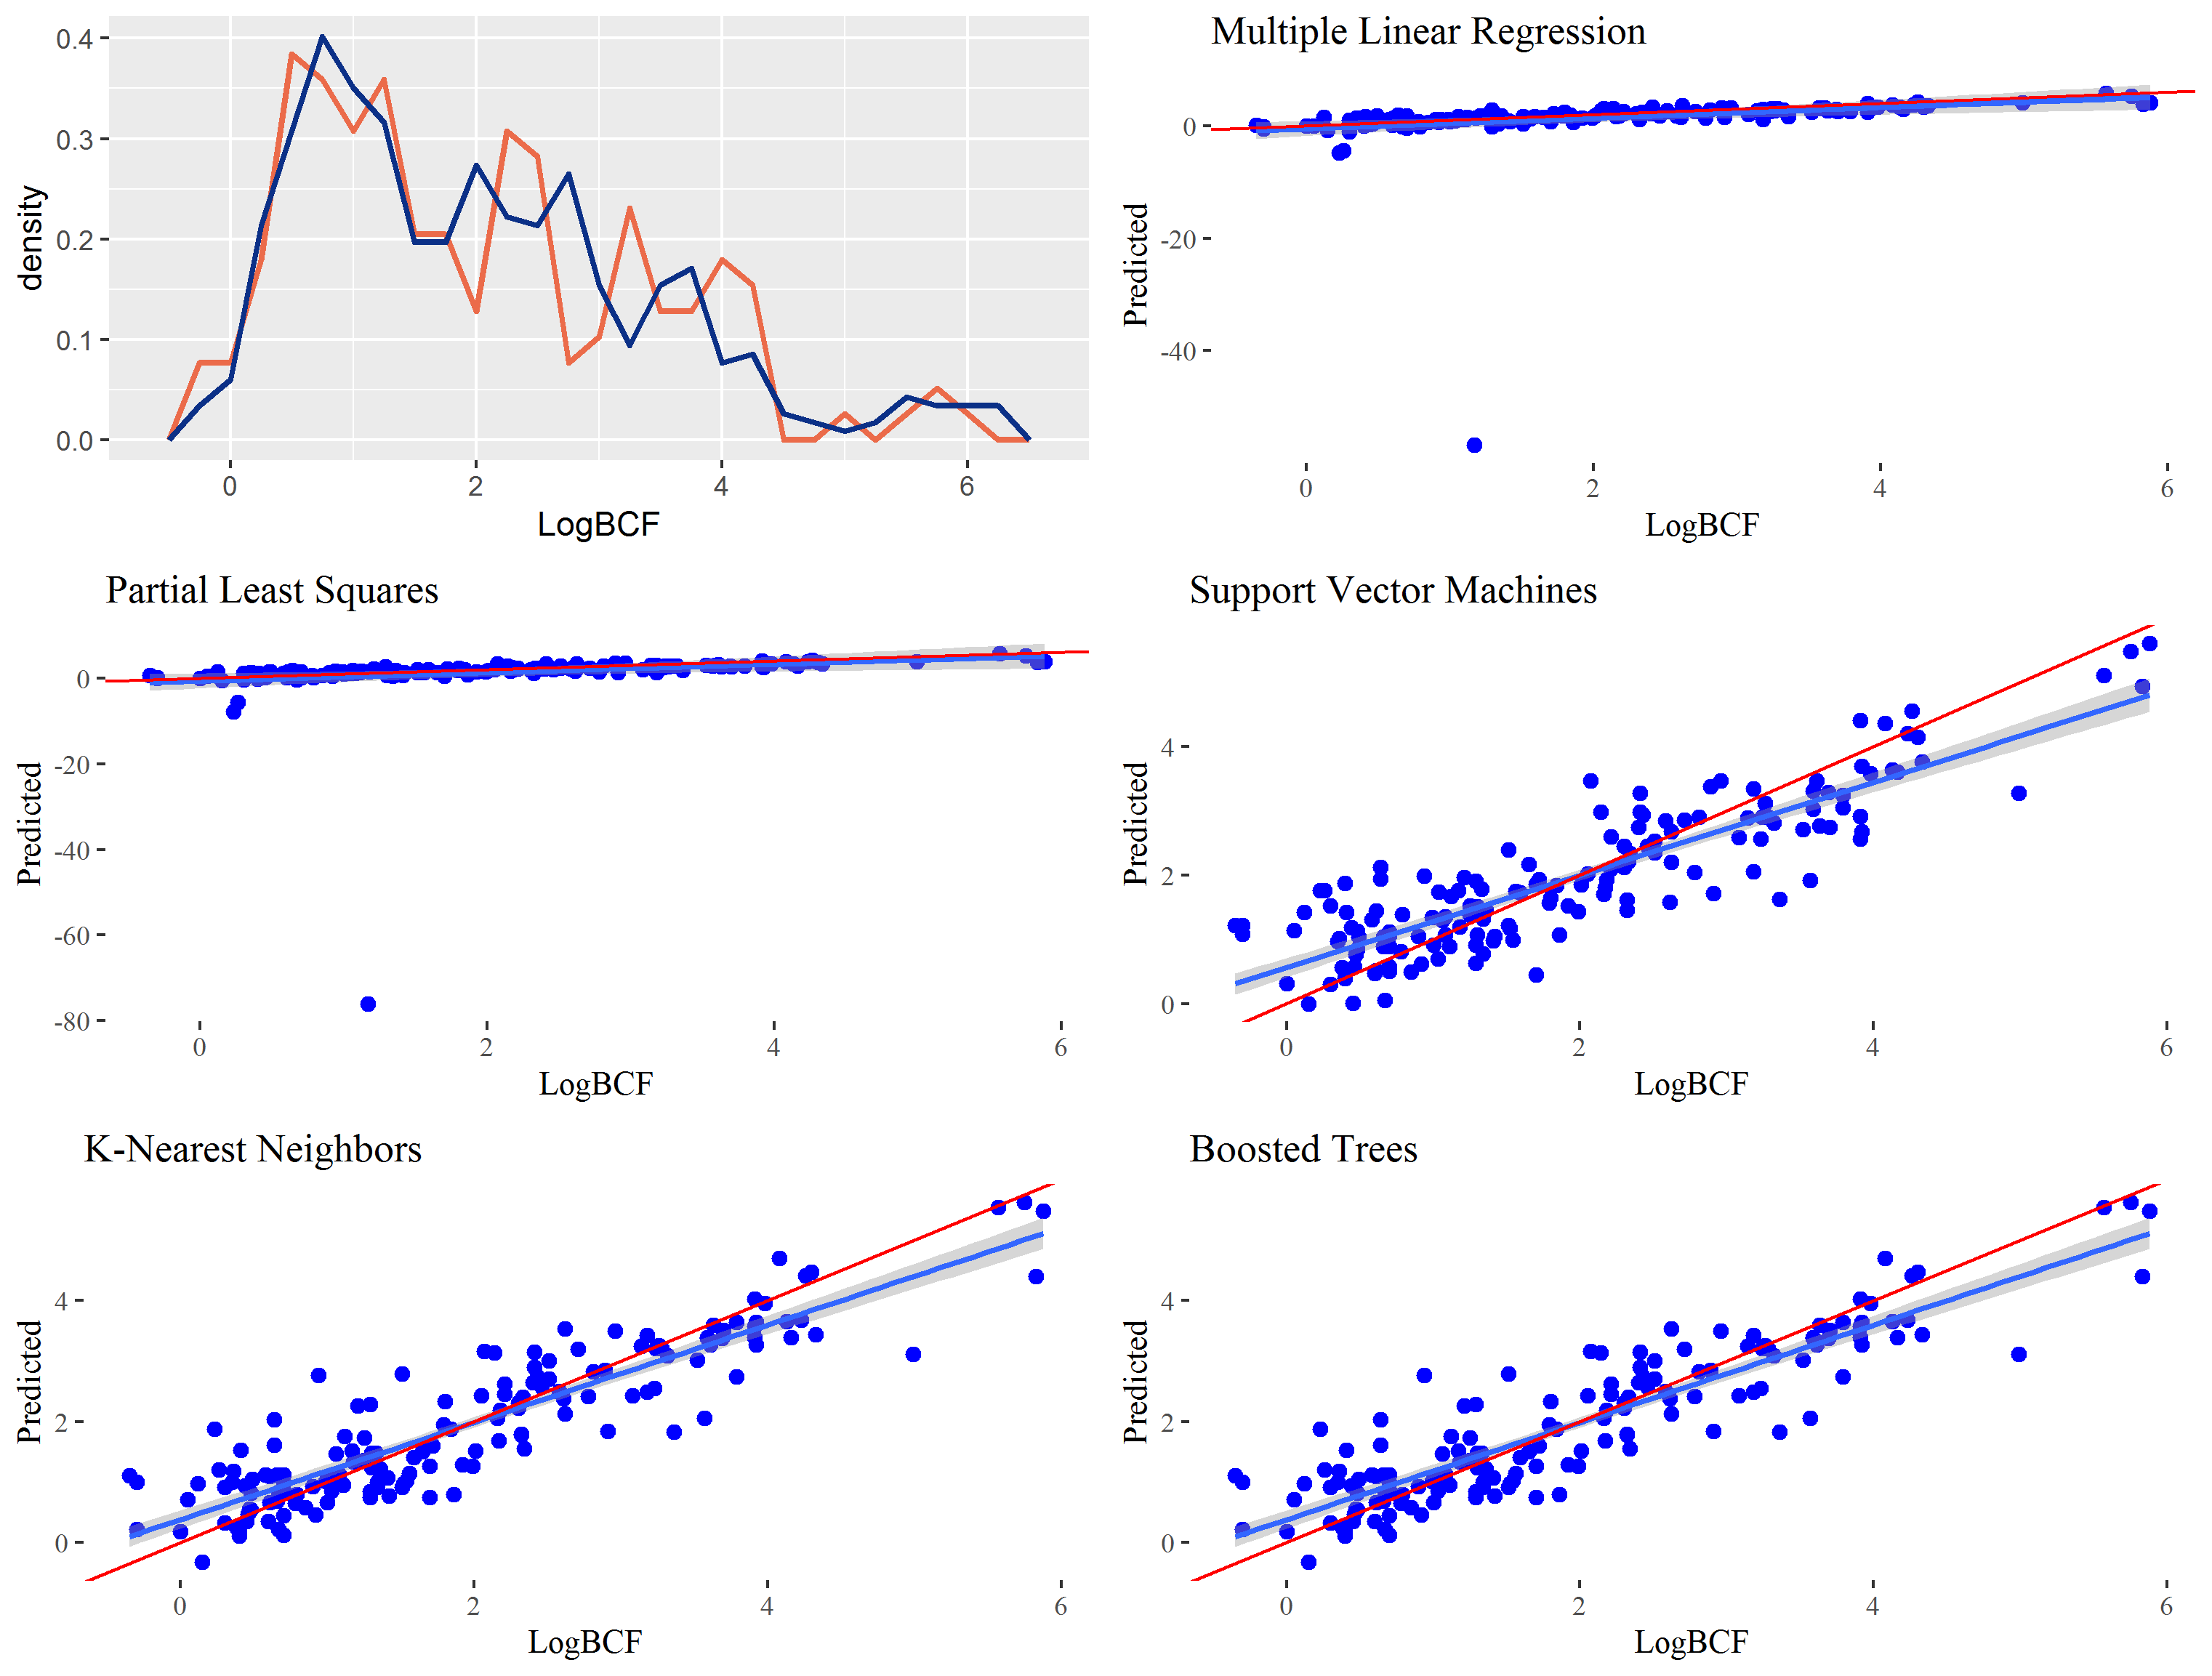
\includegraphics[width=1.0\textwidth]{BCF_plots.png}
\end{figure}

\begin{table}[H]
\begin{center}
\begin{tabular}{lrrrrr}
\toprule
% \hline
&&\\
{\bf property} & {\bf mlr} & {\bf pls} &  {\bf svm}  & {\bf kNN}  & {\bf gbm}\\
% &&\\
%\hline
\midrule
&&\\
BCF  &   0.0668 & 0.0398 & 0.7690 & 0.6916 & 0.8085\\
&&\\
\midrule
\hline
%\bottomrule
\end{tabular}
\end{center}
%\caption{Adjusted \( R^2\).}
\end{table}

\newpage
\bibliographystyle{unsrt}
\bibliography{references}

\end{document}





